\documentclass[aspectratio=169,12pt]{beamer}

\usepackage{hyperref}
\usepackage{biblatex}

\usepackage{amsmath}
\usepackage{bm}

\addbibresource{references.bib}

\usepackage{varwidth}
\usepackage{tikz}
\usetikzlibrary{tikzmark}
\usetikzlibrary{arrows}

\usepackage{multirow}
\usepackage{booktabs}
\usepackage{algorithm}
\usepackage{algpseudocode}

\usepackage{amsmath,amsthm,amssymb}
\usepackage{cleveref}
\usepackage{comment}

% Allowing page breaks in align
\allowdisplaybreaks

% Other commands
\newcommand{\loss}[1]{\ell\ifthenelse{\isempty{#1}{}}{}{\!\left(#1\right)}}
\newcommand{\negspace}[1]{\phantom{\hspace*{-#1}}}

% Math operators
\DeclareMathOperator*{\argmin}{arg\,min}
\DeclareMathOperator*{\argmax}{arg\,max}
\DeclareMathOperator*{\expect}{\mathbb{E}}
\DeclareMathOperator*{\prob}{\mathbb{P}}

% Vectors
\newcommand{\mydefv}[1]{\expandafter\newcommand\csname v#1\endcsname{\mathbf{#1}}}
\newcommand{\mydefallv}[1]{\ifx#1\mydefallv\else\mydefv{#1}\expandafter\mydefallv\fi}
\mydefallv abcekmosuvwxyz\mydefallv

% Vectors symbols
\newcommand{\mydefvsym}[1]{\expandafter\newcommand\csname v#1\endcsname{\boldsymbol{\csname #1\endcsname}}}
\newcommand{\mydefallvsym}[1]{\ifx#1\mydefallvsym\else\mydefvsym{#1}\expandafter\mydefallvsym\fi}
\mydefallvsym {sigma}{alpha}{gamma}{mu}{rho}\mydefallvsym

% Set
\newcommand{\mydefset}[1]{\expandafter\newcommand\csname set#1\endcsname{{#1}}}
\newcommand{\mydefallset}[1]{\ifx#1\mydefallset\else\mydefset{#1}\expandafter\mydefallset\fi}
\mydefallset BFHPSTVYZ\mydefallset

% Distribution over a space
\newcommand{\mydefdistr}[1]{\expandafter\newcommand\csname distr#1\endcsname{\mathcal{D}_{\csname space#1\endcsname}}}
\newcommand{\mydefalldistr}[1]{\ifx#1\mydefalldistr\else\mydefdistr{#1}\expandafter\mydefalldistr\fi}
\mydefalldistr DHNSTVXZ\mydefalldistr

% Empirical Distribution
\newcommand{\mydefedistr}[1]{\expandafter\newcommand\csname edistr#1\endcsname{\widehat{\mathcal{D}}_{\csname space#1\endcsname}}}
\newcommand{\mydefalledistr}[1]{\ifx#1\mydefalledistr\else\mydefedistr{#1}\expandafter\mydefalledistr\fi}
\mydefalledistr WZ\mydefalledistr

% Space
\newcommand{\mydefspace}[1]{\expandafter\newcommand\csname space#1\endcsname{\mathcal{#1}}}
\newcommand{\mydefallspace}[1]{\ifx#1\mydefallspace\else\mydefspace{#1}\expandafter\mydefallspace\fi}
\mydefallspace DFGHKLMNPSRTUVXYZ\mydefallspace

% Function
\newcommand{\mydeff}[1]{\expandafter\newcommand\csname f#1\endcsname[2][]{#1##1\ifthenelse{\equal{##2}{}}{}{\!\left(##2\right)}}}
\newcommand{\mydefallf}[1]{\ifx#1\mydefallf\else\mydeff{#1}\expandafter\mydefallf\fi}
\mydefallf cdfqghklsuyzCFGHKLMRT\mydefallf

% Function symbols
\newcommand{\mydeffsym}[1]{\expandafter\newcommand\csname f#1\endcsname[2][]{\csname #1\endcsname##1\ifthenelse{\equal{##2}{}}{}{\!\left(##2\right)}}}
\newcommand{\mydefallfsym}[1]{\ifx#1\mydefallfsym\else\mydeffsym{#1}\expandafter\mydefallfsym\fi}
\mydefallfsym {Omega}{phi}{epsilon}{delta}{eta}{theta}{nu}{tildeh}{kappa}{rho}\mydefallfsym

% Number Set
\newcommand{\mydefnset}[1]{\expandafter\newcommand\csname nset#1\endcsname{\mathbb{#1}}}
\newcommand{\mydefallnset}[1]{\ifx#1\mydefallnset\else\mydefnset{#1}\expandafter\mydefallnset\fi}
\mydefallnset CNRSZ\mydefallnset

% Norm
\newcommand{\normTwo}[1]{\left\|#1\right\|_2}
\newcommand{\normF}[1]{\left\|#1\right\|_\mathcal{F}}
\newcommand{\normOne}[1]{\left\|#1\right\|_1}
\newcommand{\normNuc}[1]{\left\|#1\right\|_\mathcal{*}}
\newcommand{\normMax}[1]{\left\|#1\right\|_\infty}
\newcommand{\norm}[1]{\left\|#1\right\|}
\newcommand{\abs}[1]{\left|#1\right|}
\newcommand{\hinge}[1]{\left[#1\right]_+}
\newcommand{\dotprod}[2]{\left\langle#1,#2\right\rangle}
\newcommand{\trace}[1]{\text{Tr}\left(#1\right)}
\newcommand{\inv}[1]{\left( #1 \right)^{-1}}
\newcommand{\bigO}[1]{\mathcal{O}\left( #1 \right)}

\newcommand{\scalar}[2]{\langle #1, #2 \rangle}

% Indic
\newcommand{\indic}[1]{\mathbb{I}_{ #1}}

% Ceil and Floor
\newcommand{\ceil}[1]{{\left\lceil #1 \right\rceil}}
\newcommand{\floor}[1]{{\left\lfloor #1 \right\rfloor}}

% Environments
\newtheorem{myth}{Theorem}
\newtheorem*{myth*}{Theorem}
\newtheorem{mycor}{Corollary}
\newtheorem*{mycor*}{Corollary}
\newtheorem{mylem}{Lemma}
\newtheorem*{mylem*}{Lemma}
\newtheorem{mydef}{Definition}
\newtheorem{myex}{Example}
\newtheorem*{myex*}{Example}
\newtheorem{myprop}{Proposition}

\newtheorem{myrmq}{Remark}
\newtheorem*{myrmq*}{Remark}


% Bold font in theorem headings
\makeatletter
\def\th@plain{%
  \thm@notefont{}% same as heading font
  \itshape % body font
}
\def\th@definition{%
  \thm@notefont{}% same as heading font
  \normalfont % body font
}
\makeatother
\newcommand{\targetlabel}[1][]{\fy{#1}}
\newcommand{\fairlabel}[1][]{\fs{#1}}
\newcommand{\DDP}[1][]{\text{DDP}\!\left(#1\right)}
\newcommand{\DEO}[1][]{\text{DEO}\!\left(#1\right)}
\newcommand{\eDDP}[1][]{\widehat{\text{DDP}}\!\left(#1\right)}
\newcommand{\eDEO}[1][]{\widehat{\text{DEO}}\!\left(#1\right)}
\newcommand{\eDDPm}[1][]{\widehat{\text{DDP}}^+}
\newcommand{\eDDPp}[1][]{\widehat{\text{DDP}}^-}
\newcommand{\lrDDP}[1][]{\text{LR}_{{\text{DDP}}}\!\left(#1\right)}
\newcommand{\srDDP}[1][]{\text{SR}_{{\text{DDP}}}\!\left(#1\right)}
\newcommand{\lrDEO}[1][]{\text{LR}_{{\text{DEO}}}\!\left(#1\right)}
\newcommand{\lreDDP}[1][]{\text{LR}_{\widehat{\text{DDP}}}\!\left(#1\right)}
\newcommand{\sreDDP}[1][]{\text{SR}_{\widehat{\text{DDP}}}\!\left(#1\right)}
\newcommand{\lreDEO}[1][]{\text{LR}_{\widehat{\text{DEO}}}\!\left(#1\right)}
\newcommand{\CCreDDP}[1][]{\text{CCR}_{\widehat{\text{DDP}}}\!\left(#1\right)}
\newcommand{\crDDP}[1][]{\text{R}_{\text{DDP}}\!\left(#1\right)}
\newcommand{\creDDP}[1][]{\text{R}_{\widehat{\text{DDP}}}\!\left(#1\right)}
\newcommand{\CCreDEO}[1][]{\text{CCR}_{\widehat{\text{DEO}}}\!\left(#1\right)}
\newcommand{\DDPkappa}[1][]{\text{DDP}_{\kappa}\!\left(#1\right)}
\newcommand{\DDPdelta}[1][]{\text{DDP}_{\delta}\!\left(#1\right)}
\newcommand{\eDDPkappa}[1][]{\widehat{\text{DDP}}_{\kappa}\!\left(#1\right)}
\newcommand{\eDDPdelta}[1][]{\widehat{\text{DDP}}_{\delta}\!\left(#1\right)}
\newcommand{\eDDPkappam}[1][]{\widehat{\text{DDP}}_{\kappa}^-}
\newcommand{\eDDPdeltap}[1][]{\widehat{\text{DDP}}_{\delta}^+}
\newcommand{\targeteps}{\varepsilon}
\newcommand{\faireps}{\varepsilon_f}
\newcommand{\targetmargin}{\gamma}
\newcommand{\fairnessSlack}{\mu}
\newcommand{\reasonable}{\tau}
\newcommand{\highmarginFraction}{\nu}
\newcommand{\learningProblem}{\mathrm{P}}
\newcommand{\map}[2]{\phi^{#1}\!\left(#2\right)}
\newcommand{\sign}[1]{\text{sign}\!\left(#1\right)}
\newcommand{\trueR}[1]{L\!\left(#1\right)}
\newcommand{\empR}[1]{\widehat{L}\!\left(#1\right)}
\newcommand{\reg}[1]{\fOmega{#1}}
\newcommand{\normal}[1]{\mathcal{N}\!\left(#1\right)}
\newcommand{\rad}[2]{\mathfrak{R}_{#1}\!\left(#2\right)}

\newcommand{\fairscalar}[1][]{\fq{#1}}
\newcommand{\phimax}{\phi_{\mathrm{max}}}

\newcommand{\cause}[1]{&{\color{gray}\downarrow{}\;{\small \text{#1}}} \nonumber\\}

\newcommand{\priv}{\mathrm{priv}}
\newcommand{\refer}{\mathrm{ref}}


% accuracy
\DeclareMathOperator*{\Acc}{Acc}

%%% Local Variables:
%%% mode: latex
%%% TeX-master: "main"
%%% End:

%%%%%%%%%%%%%%%%%%%%%%%%%%%%%%%%%%%%%%%%%%%%%%%%%%%%%%%%%%%%%%%%%%%%%%%%%%%%%%%
% Style mathbb
%%%%%%%%%%%%%%%%%%%%%%%%%%%%%%%%%%%%%%%%%%%%%%%%%%%%%%%%%%%%%%%%%%%%%%%%%%%%%%%

% cal letters
\newcommand{\cA}{\mathcal{A}}
\newcommand{\cB}{\mathcal{B}}
\newcommand{\cC}{\mathcal{C}}
\newcommand{\cD}{\mathcal{D}}
\newcommand{\cE}{\mathcal{E}}
\newcommand{\cF}{\mathcal{F}}
\newcommand{\cG}{\mathcal{G}}
\newcommand{\cH}{\mathcal{H}}
\newcommand{\cI}{\mathcal{I}}
\newcommand{\cJ}{\mathcal{J}}
\newcommand{\cK}{\mathcal{K}}
\newcommand{\cL}{\mathcal{L}}
\newcommand{\cM}{\mathcal{M}}
\newcommand{\cN}{\mathcal{N}}
\newcommand{\cO}{\mathcal{O}}
\newcommand{\cP}{\mathcal{P}}
\newcommand{\cQ}{\mathcal{Q}}
\newcommand{\cR}{\mathcal{R}}
\newcommand{\cS}{\mathcal{S}}
\newcommand{\cT}{\mathcal{T}}
\newcommand{\cU}{\mathcal{U}}
\newcommand{\cV}{\mathcal{V}}
\newcommand{\cW}{\mathcal{W}}
\newcommand{\cX}{\mathcal{X}}
\newcommand{\cY}{\mathcal{Y}}
\newcommand{\cZ}{\mathcal{Z}}

% bold letters (upper case)
\newcommand{\bfA}{\mathbf{A}}
\newcommand{\bfB}{\mathbf{B}}
\newcommand{\bfC}{\mathbf{C}}
\newcommand{\bfD}{\mathbf{D}}
\newcommand{\bfE}{\mathbf{E}}
\newcommand{\bfF}{\mathbf{F}}
\newcommand{\bfG}{\mathbf{G}}
\newcommand{\bfH}{\mathbf{H}}
\newcommand{\bfI}{\mathbf{I}}
\newcommand{\bfJ}{\mathbf{J}}
\newcommand{\bfK}{\mathbf{K}}
\newcommand{\bfL}{\mathbf{L}}
\newcommand{\bfM}{\mathbf{M}}
\newcommand{\bfN}{\mathbf{N}}
\newcommand{\bfO}{\mathbf{O}}
\newcommand{\bfP}{\mathbf{P}}
\newcommand{\bfQ}{\mathbf{Q}}
\newcommand{\bfR}{\mathbf{R}}
\newcommand{\bfS}{\mathbf{S}}
\newcommand{\bfT}{\mathbf{T}}
\newcommand{\bfU}{\mathbf{U}}
\newcommand{\bfV}{\mathbf{V}}
\newcommand{\bfW}{\mathbf{W}}
\newcommand{\bfX}{\mathbf{X}}
\newcommand{\bfY}{\mathbf{Y}}
\newcommand{\bfZ}{\mathbf{Z}}

% bold letters (lower case)
\newcommand{\bfa}{\mathbf{a}}
\newcommand{\bfb}{\mathbf{b}}
\newcommand{\bfc}{\mathbf{c}}
\newcommand{\bfd}{\mathbf{d}}
\newcommand{\bfe}{\mathbf{e}}
\newcommand{\bfbf}{\mathbf{f}}
\newcommand{\bfg}{\mathbf{g}}
\newcommand{\bfh}{\mathbf{h}}
\newcommand{\bfi}{\mathbf{i}}
\newcommand{\bfj}{\mathbf{j}}
\newcommand{\bfk}{\mathbf{k}}
\newcommand{\bfl}{\mathbf{l}}
%\newcommand{\fbm}{\mathbf{m}} % not compatible with bm package.
\newcommand{\bfn}{\mathbf{n}}
\newcommand{\bfo}{\mathbf{o}}
\newcommand{\bfp}{\mathbf{p}}
\newcommand{\bfq}{\mathbf{q}}
\newcommand{\bfr}{\mathbf{r}}
\newcommand{\bfs}{\mathbf{s}}
\newcommand{\bft}{\mathbf{t}}
\newcommand{\bfu}{\mathbf{u}}
\newcommand{\bfv}{\mathbf{v}}
\newcommand{\bfw}{\mathbf{w}}
\newcommand{\bfx}{\mathbf{x}}
\newcommand{\bfy}{\mathbf{y}}
\newcommand{\bfz}{\mathbf{z}}

% bold greek letters
\newcommand{\bbeta}{{\boldsymbol\beta}}
\newcommand{\bmu}{{\boldsymbol\mu}}
\newcommand{\bxi}{{\boldsymbol\xi}}
\newcommand{\btheta}{\boldsymbol{\theta}}
\newcommand{\balpha}{\boldsymbol{\alpha}}
\newcommand\bSigma{{\boldsymbol\Sigma}}
\newcommand\bOmega{{\boldsymbol\Omega}}
\newcommand{\beps}{{\boldsymbol\eps}}
\newcommand{\bepsilon}{{\boldsymbol\varepsilon}}
\newcommand{\bfepsilon}{{\boldsymbol\varepsilon}}
\newcommand{\bftheta}{{\boldsymbol\theta}}
\newcommand{\bfbeta}{{\boldsymbol\beta}}

% bb letters
\newcommand{\bbA}{\mathbb{A}}
\newcommand{\bbB}{\mathbb{B}}
\newcommand{\bbC}{\mathbb{C}}
\newcommand{\bbD}{\mathbb{D}}
\newcommand{\bbE}{\mathbb{E}}
\newcommand{\bbF}{\mathbb{F}}
\newcommand{\bbG}{\mathbb{G}}
\newcommand{\bbH}{\mathbb{H}}
%\newcommand{\bbI}{\mathbb{I}}
\newcommand{\bbI}{\mathds{1}}
\newcommand{\bbJ}{\mathbb{J}}
\newcommand{\bbK}{\mathbb{K}}
\newcommand{\bbL}{\mathbb{L}}
\newcommand{\bbM}{\mathbb{M}}
\newcommand{\bbN}{\mathbb{N}}
\newcommand{\bbO}{\mathbb{O}}
\newcommand{\bbP}{\mathbb{P}}
\newcommand{\bbQ}{\mathbb{Q}}
\newcommand{\bbR}{\mathbb{R}}
\newcommand{\bbS}{\mathbb{S}}
\newcommand{\bbT}{\mathbb{T}}
\newcommand{\bbU}{\mathbb{U}}
\newcommand{\bbV}{\mathbb{V}}
\newcommand{\bbW}{\mathbb{W}}
\newcommand{\bbX}{\mathbb{X}}
\newcommand{\bbY}{\mathbb{Y}}
\newcommand{\bbZ}{\mathbb{Z}}

%% number spaces
\newcommand{\RR}{\mathbb{R}}



% latin
\newcommand{\ie}{{\em i.e.,~}}
\newcommand{\etal}{{\em et al.~}}
\newcommand{\eg}{{\em e.g.,~}}
\newcommand{\lcf}{{\em cf.~}}
\newcommand{\rem}{\underline{Rem}:~}
\newcommand{\iid}{\textit{i.i.d.}}
\newcommand{\VA}{\textit{v.a.}~}



%%% Local Variables:
%%% mode: latex
%%% TeX-master: "main"
%%% End:


\definecolor{darkspringgreen}{rgb}{0.09, 0.45, 0.27}
\makeatletter
\newcommand{\Pause}[1][]{\unless\ifmeasuring@\relax
\pause[#1]%
\fi}
\makeatother
%%%%%% Template things

% space between paragraphs
\parskip=1em

% title font
\setbeamerfont{title}{size=\Large}%, series=\bfseries}
\setbeamerfont{frametitle}{size=\LARGE}%, series=\bfseries}
\setbeamerfont{institute}{size=\normalsize}%, series=\bfseries}

% spacing between frame title and content
\addtobeamertemplate{frametitle}{\vspace*{0.2cm}}{\vspace*{0.5cm}}

% color
\definecolor{beamer@blendedblue}{rgb}{0.8, 0, 0.34}%{0.44, 0.16, 0.39}

% no navigation
\beamertemplatenavigationsymbolsempty

% slide numbers
\setbeamertemplate{footline}
{
  \hbox{\begin{beamercolorbox}[wd=1\paperwidth,ht=5.25ex,dp=4ex,right]{framenumber}%
      \large \insertframenumber{}~~
    \end{beamercolorbox}}%
  \vskip0pt%
}

% centered titles
\makeatletter
\long\def\beamer@@frametitle[#1]#2{%
  \beamer@ifempty{#2}{}{%
    \gdef\insertframetitle{\centering{#2\ifnum\beamer@autobreakcount>0\relax{}\space\usebeamertemplate*{frametitle continuation}\fi}}%
  \gdef\beamer@frametitle{#2}%
  \gdef\beamer@shortframetitle{#1}%
}%
}
\makeatother

%%%%% Equations

\newcounter{mytn}
\makeatletter
\newcommand{\tmn}[3][]{\stepcounter{mytn}%
\tikzmarknode[Col\the\numexpr\value{mytn}-\mytn@start\relax/.try,inner xsep=2pt,%
minimum height=1.6em,inner sep=2mm,#1]{mytn-\number\value{mytn}}{#2}%
\expandafter\gdef\csname tmn@annot@\number\value{mytn}\endcsname{#3}}
\newenvironment{AnnotatedEquation}{\edef\mytn@start{\number\value{mytn}}%
\begin{equation*}}{\end{equation*}%
\edef\mytn@end{\number\value{mytn}}%
\ifnum\mytn@end>\mytn@start
\begin{itemize}
 \foreach \X in {\the\numexpr\mytn@start+1,...,\mytn@end}
 {\item \tikzmarknode{mytn-annot-\X}{\csname tmn@annot@\X\endcsname}%
   \begin{tikzpicture}[overlay,remember picture]
  \draw[-stealth] (mytn-annot-\X.east) to[out=0,in=-90] (mytn-\X.south);
 \end{tikzpicture}}
\end{itemize}
\fi}
\makeatother
\tikzset{ Col1/.style= {fill=blue!20,anchor=base,rounded corners=2pt},
Col2/.style= {Col1, fill=red!20},
Col3/.style= {Col1, fill=green!20},
Col4/.style= {Col1, fill=yellow!20},
}

%%%%% INFORMATION

\title{Federated Reinforcement Learning for Decision Making}
\author{
  \vspace{-0.5em}
  Paul Mangold\\[1em]
  CMAP, École Polytechnique, France
  \vspace{-1em}
}
\titlegraphic{
  \vspace{-1em}
  
\includegraphics[height=4em]{logos/x.pdf}\qquad\qquad\qquad%
  
\includegraphics[height=4em]{logos/tii.pdf}
  \vspace{-1.5em}
}
\institute{}
\date{October 2, 2024}

%%%%% DOCUMENT

\begin{document}

%% TITLE PAGE

\begin{frame}[plain]
  \titlepage
\end{frame}
\addtocounter{framenumber}{-1}

\begin{frame}
  \begin{center}
    \textcolor{beamer@blendedblue}{
      \huge Background on \\[1em]
      \huge Federated Learning
    }
  \end{center}
\end{frame}

\begin{frame}{Data Collection}
  \hspace{-3em}
  \begin{minipage}{0.5\linewidth}
    \begin{center}
      Data center\\[0.5em]
      
      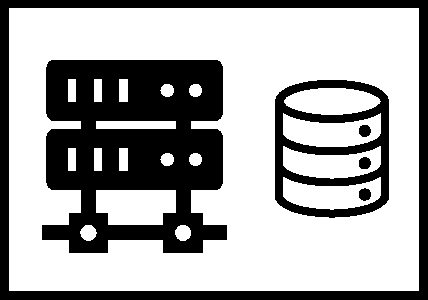
\includegraphics[width=0.4\linewidth]{images/central.pdf}
    \end{center}
    
  \end{minipage}\pause vs.\hspace{1.5em}%
  \begin{minipage}{0.5\linewidth}
    \pause
    \begin{center}
      Data collection \emph{by users} \\[0.5em]
      
      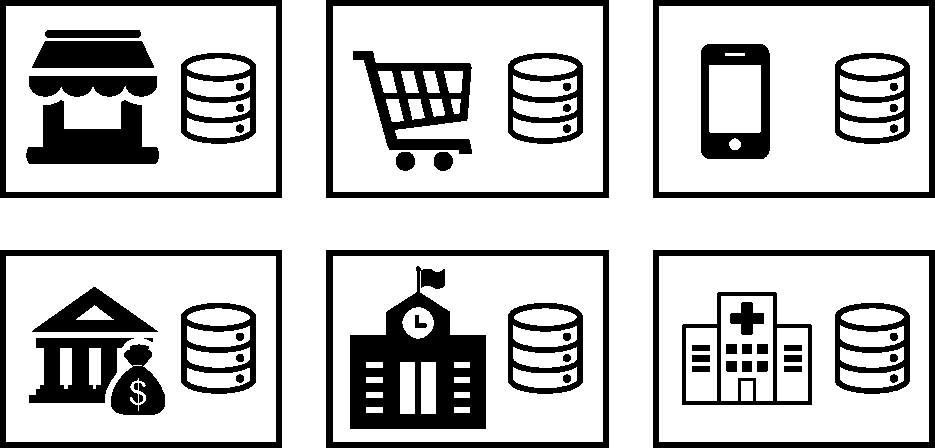
\includegraphics[width=0.8\linewidth]{images/decentralized.pdf}
    \end{center}
  \end{minipage}

  \vspace{1em}

  \pause
  
  \begin{center}
    \textbf{
    $\rightarrow$ how to use all this data?}
  \end{center}
\end{frame}


\begin{frame}{Classical Machine Learning}
  
  \begin{minipage}{0.4\linewidth}
    \begin{center}
      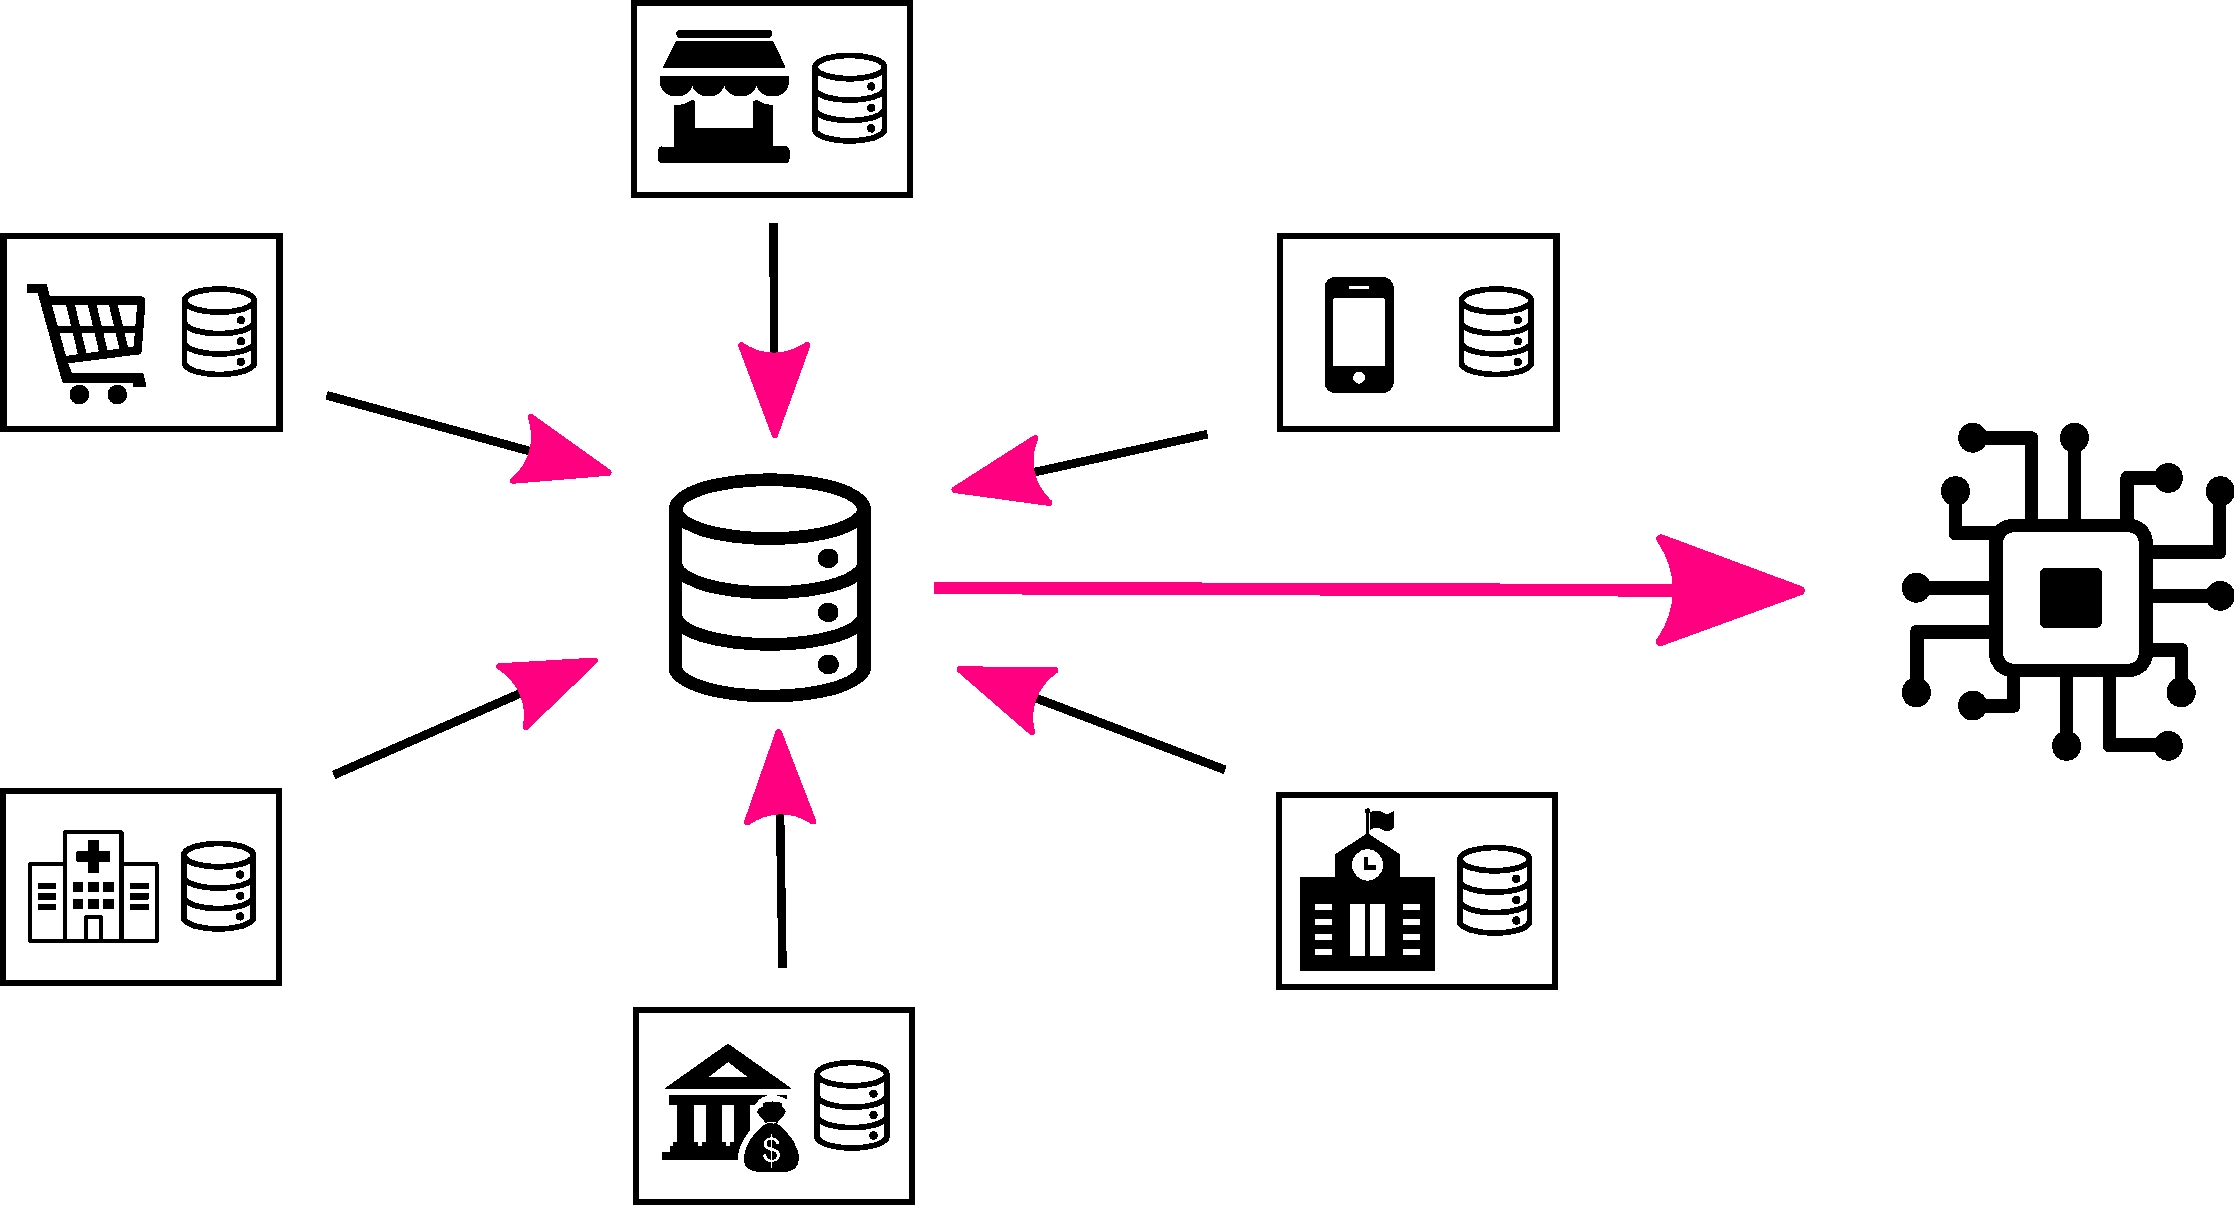
\includegraphics[width=\linewidth]{images/centralize-data.pdf}
    \end{center}
    
  \end{minipage}~~~~%
  \begin{minipage}{0.5\linewidth}
    \pause
    \begin{center}
      A single optimization problem      
    \end{center}
    \begin{align*}
      \min_{\theta \in \mathbb{R}^d} \mathbb{E}_{x, y \sim D} \Big[ \ell( \theta; x, y ) \Big]
    \end{align*}

    \begin{center}
      (e.g. empirical risk minimization)
    \end{center}
    
  \end{minipage}
\end{frame}

\begin{frame}[t]{Centralizing in a data center is difficult}

  Centralizing data is often impossible
  \begin{itemize}
  \item \emph{Privacy}:

    {\small
    $\rightarrow$ data may be sensitive (e.g. health records, geolocation)
    }
    \\
    ~

  \item \emph{Volume of data}:

    {\small
      $\rightarrow$ data may be large (e.g. cameras of self-driving car)
    }
    \\
    ~
    

    
  \end{itemize}

\end{frame}



\begin{frame}{Why share in the first place?}

  If it is so difficult to share data... why do it?
  \begin{itemize}
  \item Local datasets are often too small

    {\small
      $\rightarrow$ no statistical significance (e.g. medical study)
    }
    \\
    ~
    
    
  \item Local datasets can be biased

    {\small
      $\rightarrow$ if a self-driving car learns in countryside, can it drive in the city?
    }
    \\
    ~
    
        
  \end{itemize}
  
\end{frame}

\begin{frame}{Federated Learning}
  
  \begin{minipage}{0.4\linewidth}
    \begin{center}
      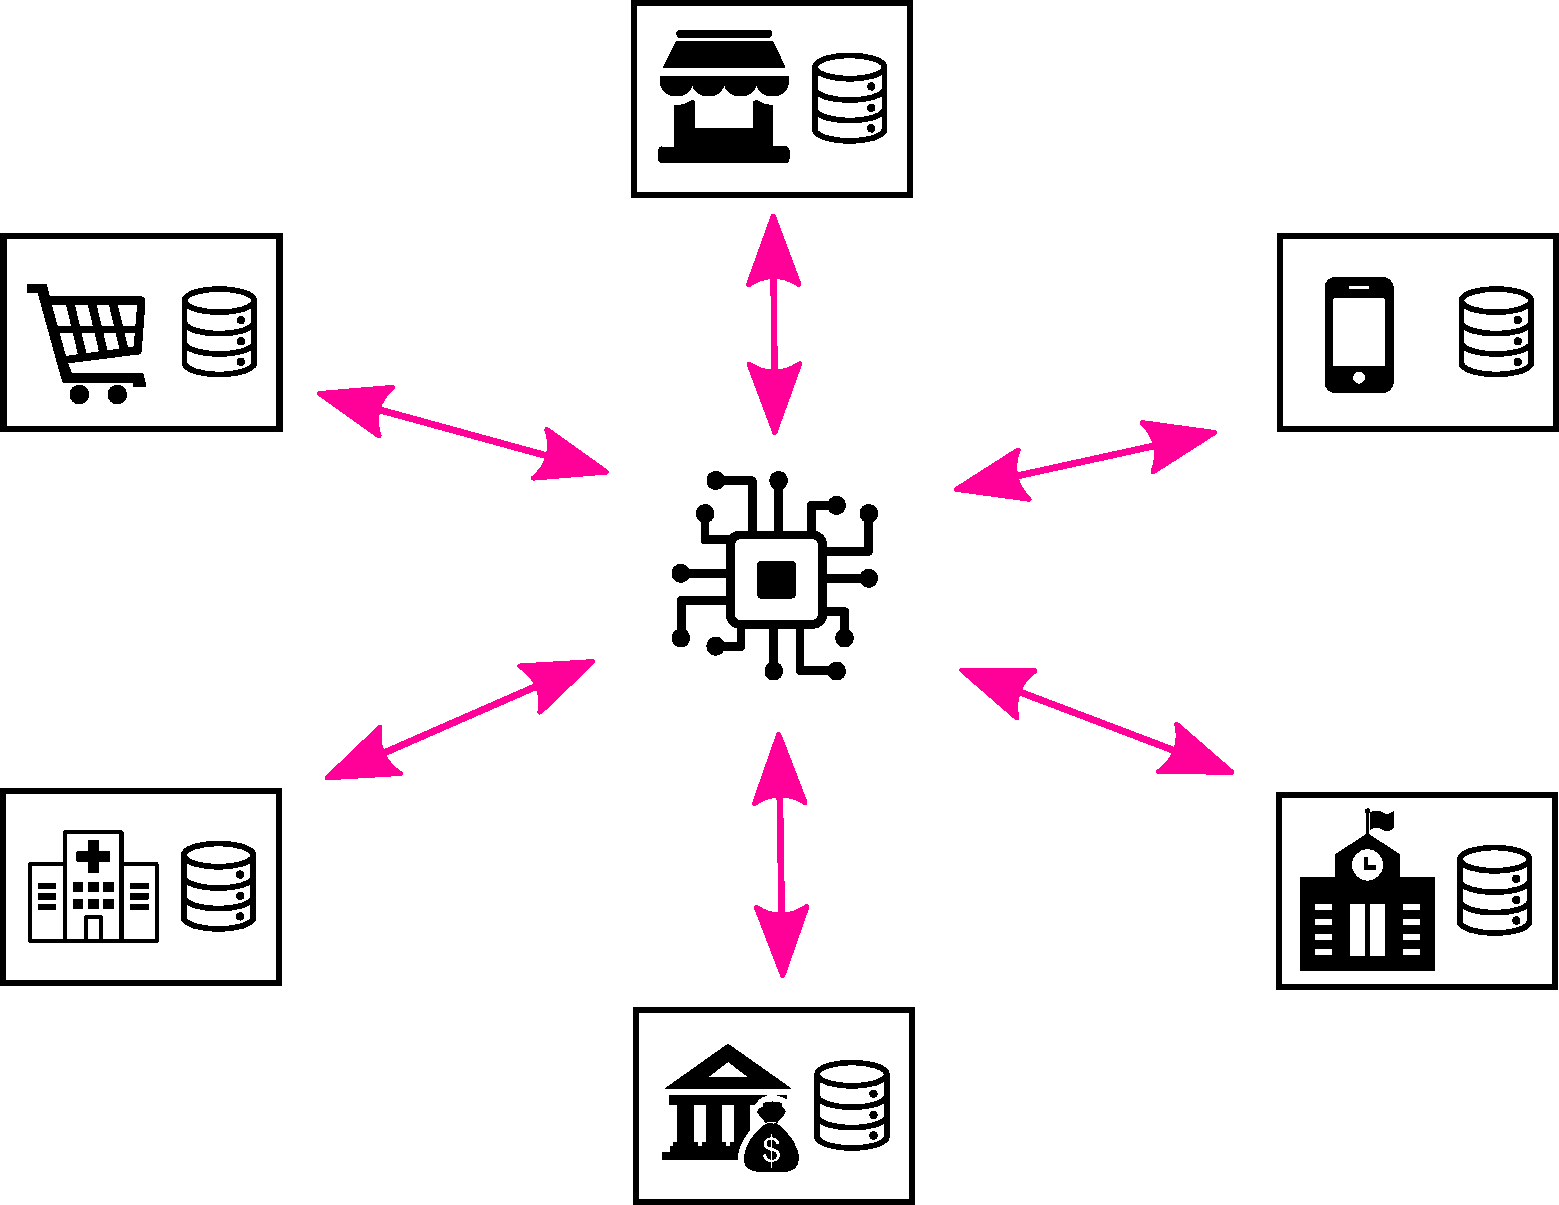
\includegraphics[width=\linewidth]{images/federated-training.pdf}
    \end{center}
    
  \end{minipage}~~~~%
  \pause
  \begin{minipage}{0.5\linewidth}
    \begin{center}
      Multiple sub-problems
      \begin{align*}
        \min_{\theta \in \mathbb{R}^d} 
        \sum_{c=1}^N \mathbb{E}_{x^c, y^c \sim D^c} \Big[ \ell( \theta; x^c, y^c ) \Big]
      \end{align*}
      
      $\rightarrow$ but only \emph{one shared solution}
    \end{center}
    
  \end{minipage}

%  \only<2>{%
%    \tikz[overlay,remember picture]
%    \node[fill=beamer@blendedblue!10,text=black,inner sep=2em,line width=2pt,draw=beamer@blendedblue] at ([xshift=0cm,yshift=0cm]current page.center){\LARGE $\rightarrow$ What about Federated RL?};
%  }  
\end{frame}


\begin{frame}[t]{Federated Optimization}
  \vspace{-2em}
  \begin{align*}
    \theta_\star \in \arg\min_{\theta \in \mathbb{R}^d} 
    \sum_{c=1}^N f^c(\theta)
    \enspace,
    \quad
    \text{ where }
    f^c(\theta) = \mathbb{E}_{x^c, y^c \sim D^c} \Big[ \ell( \theta; x^c, y^c ) \Big]
  \end{align*}

  \pause
  

  Federated Averaging (or local (S)GD)\footfullcite{mcmahan2017communication}

  \vspace{-0.5em}
  
  \begin{itemize}
  \item For each $t = 0 ...$ :
    \begin{itemize}
      \normalsize
    \item Set $\theta_{t,0}^c = \theta_t$
    \item For each agent $c$, do $K$ gradient updates: \\[0.5em]
      
      \begin{center}
        $\theta_{t,k+1}^c = \theta_{t,k}^c - \eta \nabla f^c( \theta_{t,k}^c )$
      \end{center}
      
      \vspace{0.5em}
      
    \end{itemize}
  \item Aggregate models: $\theta_{t+1} = \frac{1}{N} \sum_{c=1}^N \theta_{t,K}^c$
  \end{itemize}

  \vspace{1.5em}

\end{frame}



%\begin{frame}{Communication and Sample Complexity\\[-0.5em]
%  \large I - Homogeneous Data}
  
%\end{frame}


%\begin{frame}{Communication and Sample Complexity\\[-0.5em]
%  \large II - Heterogeneous Data}
  
%\end{frame}

\begin{frame}{Communication and Sample Complexity\\[-0.5em]
    \large Local Training vs. Precision}
  
  \vspace{-1em}
  
  \begin{center}
    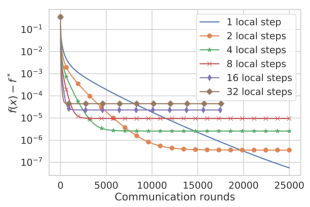
\includegraphics[width=0.6\linewidth]{images/comm-vs-local.pdf}
  \end{center}

  \vspace{-1em}

  \footnotesize
  (Figure from \fullcite{khaeld20tighter})
\end{frame}


\begin{frame}{Centralizing in a data center is difficult\\[-0.5em]
  \normalsize ... continued!}

  Centralizing data is often impossible
  \begin{itemize}
  \item \emph{Privacy}:

    {\small
    $\rightarrow$ data may be sensitive (e.g. health records, geolocation)
    }
    \\
    ~

  \item \emph{Volume of data}:

    {\small
      $\rightarrow$ data may be large (e.g. cameras of self-driving car)
    }
    \\
    ~

    \pause
    
  \item \color{red} \textbf{Time}: 

    \color{red}
    
    \textbf{\small
        $\rightarrow$ it may be needed to take decisions on the go $\rightarrow$ reinforcement learning!
      }

    
  \end{itemize}

\end{frame}






\begin{frame}
  \begin{center}
    \textcolor{beamer@blendedblue}{
      \huge Federated \\[1em]
      \huge Reinforcement Learning
    }
  \end{center}
\end{frame}

\begin{frame}
  \begin{center}
    Take $N$ environments (``Markov Decision Processes'')
  \end{center}

  \begin{center}
    \resizebox{!}{17em}{
          \begin{tikzpicture}[->,>=stealth',auto,node distance=3cm,
  thick,main node/.style={circle,draw,font=\sffamily\Large\bfseries}]
% nodes 
    \node[draw,fill=white, align=center, inner sep=5pt] (A1) at (0, 1.5) {agent 1 \\ $s_t^{(1)}$};
    \node[draw, fill=white, align=center, inner sep=5pt] (B1) at (0, 0) {env 1};

    
    \node[draw,fill=white, align=center, inner sep=5pt] (A2) at (0, -1.5) {agent 2 \\ $s_t^{(2)}$};
    \node[draw, fill=white, align=center, inner sep=5pt] (B2) at (0, -3) {env 2};

    \node (dots) at (0, -4) {$\cdots$};
    
    \node[draw,fill=white, align=center, inner sep=5pt] (An) at (0, -5.5) {agent n \\ $s_t^{(n)}$};
    \node[draw, fill=white, align=center, inner sep=5pt] (Bn) at (0, -7) {env n};


% arrows
\draw [->] (B1.west) to [out=180,in=180] (A1.west) ;
\draw [->] (A1.east) to [out=0,in=0] (B1.east);
\draw [->] (B2.west) to [out=180,in=180] (A2.west) ;
\draw [->] (A2.east) to [out=0,in=0] (B2.east);
\draw [->] (Bn.west) to [out=180,in=180] (An.west) ;
\draw [->] (An.east) to [out=0,in=0] (Bn.east);

\node[align=center,inner sep=15pt] (A1t) at (-1.7, 0.75) {$r_t^{(1)}$ \\[0.5em] $S_{t+1}^{(1)}$};
\node[align=center,inner sep=15pt] (B1t) at (1.8, 0.75) {$a_t^{(1)}$};
\node[align=center,inner sep=15pt] (C1t) at (-4, 0.75) {
\includegraphics[width=4em]{images/sedan-car-icon.pdf}};

\node[align=center,inner sep=15pt] (A2t) at (-1.7, -2.25) {$r_t^{(2)}$ \\[0.5em] $S_{t+1}^{(2)}$};
\node[align=center,inner sep=15pt] (B2t) at (1.8, -2.25) {$a_t^{(2)}$};

\node[align=center,inner sep=15pt] (C2t) at (-4, -2.25) {
\includegraphics[width=4em]{images/logistic-van-icon.pdf}};


\node[align=center,inner sep=15pt] (Ant) at (-1.7, -6.25) {$r_t^{(n)}$ \\[0.5em] $S_{t+1}^{(n)}$};
\node[align=center,inner sep=15pt] (Bnt) at (1.8, -6.25) {$a_t^{(n)}$};

\node[align=center,inner sep=15pt] (Cnt) at (-4, -6.25)  {
\includegraphics[width=4em]{images/suv-car-icon.pdf}};

\end{tikzpicture}   
%%% Local Variables:
%%% mode: LaTeX
%%% TeX-master: "main"
%%% End:

    }
\end{center}
\end{frame}

\begin{frame}[t]{Some Formalism...}
  For agent $c = 1 .. N$, with shared policy $\pi$
  \begin{gather*}
    S_0^c = s, \\
    \only<2,3,4,5>{
      A_h^c \sim \pi(\cdot | S_t^c),
      \\
    }%
    \only<3,4,5>{
    S_{h+1}^c \sim P^c_{\text{MDP}}(\cdot| S_t^c,A_t^c)
    }%
  \end{gather*}

  \pause
  \pause
  \pause
  
  For a given state $s \in \mathcal{S}$, \textcolor{beamer@blendedblue}{\bfseries value of the policy} for agent $c \in [N]$:
  \begin{align*}
    V^{c,\pi}(s) = \textstyle{\mathbb{E}\left[\sum_{t=0}^{H} r^{c}(S_t^c,A_t^c)\right]}
  \end{align*}
  where $H$ is the horizon (length of episode) and $r^c$ is the reward

  \only<5>{%
    \tikz[overlay,remember picture]
    \node[fill=beamer@blendedblue!10,text=black,inner sep=2em,line width=2pt,draw=beamer@blendedblue] at ([xshift=0cm,yshift=1.5cm]current page.center){\LARGE Goal: learn $\pi$ with highest value!};
  }  

\end{frame}


\begin{frame}
  \begin{center}
    Take $N$ environments (``Markov Decision Processes'')
  \end{center}

  \begin{center}
    \resizebox{!}{17em}{
          \begin{tikzpicture}[->,>=stealth',auto,node distance=3cm,
  thick,main node/.style={circle,draw,font=\sffamily\Large\bfseries}]
% nodes 
    \node[draw,fill=white, align=center, inner sep=5pt] (A1) at (0, 1.5) {agent 1 \\ $s_t^{(1)}$};
    \node[draw, fill=white, align=center, inner sep=5pt] (B1) at (0, 0) {env 1};

    
    \node[draw,fill=white, align=center, inner sep=5pt] (A2) at (0, -1.5) {agent 2 \\ $s_t^{(2)}$};
    \node[draw, fill=white, align=center, inner sep=5pt] (B2) at (0, -3) {env 2};

    \node (dots) at (0, -4) {$\cdots$};
    
    \node[draw,fill=white, align=center, inner sep=5pt] (An) at (0, -5.5) {agent n \\ $s_t^{(n)}$};
    \node[draw, fill=white, align=center, inner sep=5pt] (Bn) at (0, -7) {env n};


% arrows
\draw [->] (B1.west) to [out=180,in=180] (A1.west) ;
\draw [->] (A1.east) to [out=0,in=0] (B1.east);
\draw [->] (B2.west) to [out=180,in=180] (A2.west) ;
\draw [->] (A2.east) to [out=0,in=0] (B2.east);
\draw [->] (Bn.west) to [out=180,in=180] (An.west) ;
\draw [->] (An.east) to [out=0,in=0] (Bn.east);

\node[align=center,inner sep=15pt] (A1t) at (-1.7, 0.75) {$r_t^{(1)}$ \\[0.5em] $S_{t+1}^{(1)}$};
\node[align=center,inner sep=15pt] (B1t) at (1.8, 0.75) {$a_t^{(1)}$};
\node[align=center,inner sep=15pt] (C1t) at (-4, 0.75) {
\includegraphics[width=4em]{images/sedan-car-icon.pdf}};

\node[align=center,inner sep=15pt] (A2t) at (-1.7, -2.25) {$r_t^{(2)}$ \\[0.5em] $S_{t+1}^{(2)}$};
\node[align=center,inner sep=15pt] (B2t) at (1.8, -2.25) {$a_t^{(2)}$};

\node[align=center,inner sep=15pt] (C2t) at (-4, -2.25) {
\includegraphics[width=4em]{images/logistic-van-icon.pdf}};


\node[align=center,inner sep=15pt] (Ant) at (-1.7, -6.25) {$r_t^{(n)}$ \\[0.5em] $S_{t+1}^{(n)}$};
\node[align=center,inner sep=15pt] (Bnt) at (1.8, -6.25) {$a_t^{(n)}$};

\node[align=center,inner sep=15pt] (Cnt) at (-4, -6.25)  {
\includegraphics[width=4em]{images/suv-car-icon.pdf}};

\node[fill=white, align=center, inner sep=5pt] (model) at (12, -2.7) {global policy};

\node[draw, fill=white, align=center, inner sep=24pt] (algo) at (7, -2.7) {central server};
% arrows
\draw[<->] (B1t) to (algo);
\draw[<->] (B2t) to (algo);
\draw[<->] (Bnt) to (algo);
\draw[->] (algo) to (model);

\end{tikzpicture}   
%%% Local Variables:
%%% mode: LaTeX
%%% TeX-master: "main"
%%% End:

    }
\end{center}
\end{frame}


\begin{frame}{Federated Reinforcement Learning!}
  \begin{center}
    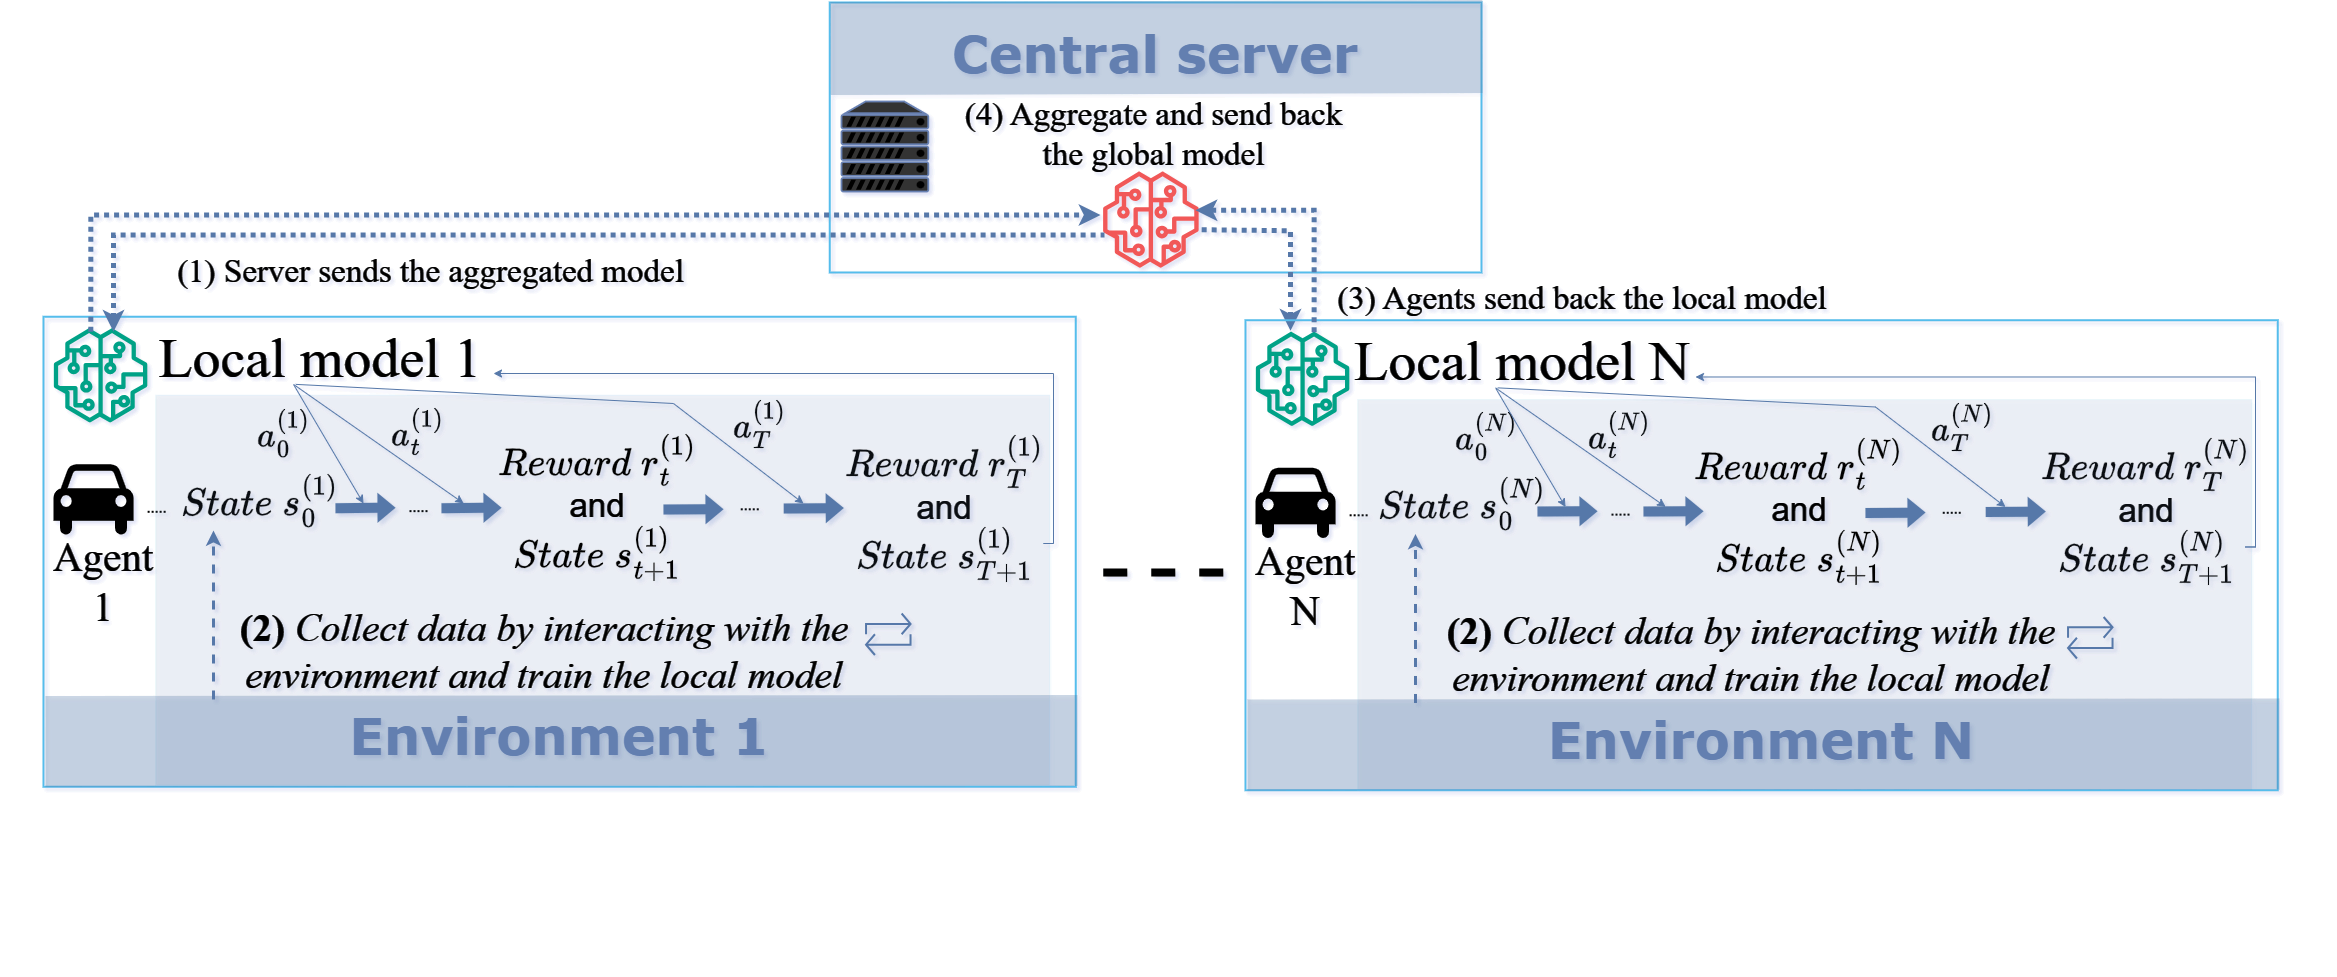
\includegraphics[width=\linewidth]{img/feddrldiag0.drawio.png}
  \end{center}
\end{frame}



\begin{frame}{Example: CartPole}
  \qquad
  \begin{minipage}[t]{0.3\linewidth}
    
  \begin{figure}
    \centering
    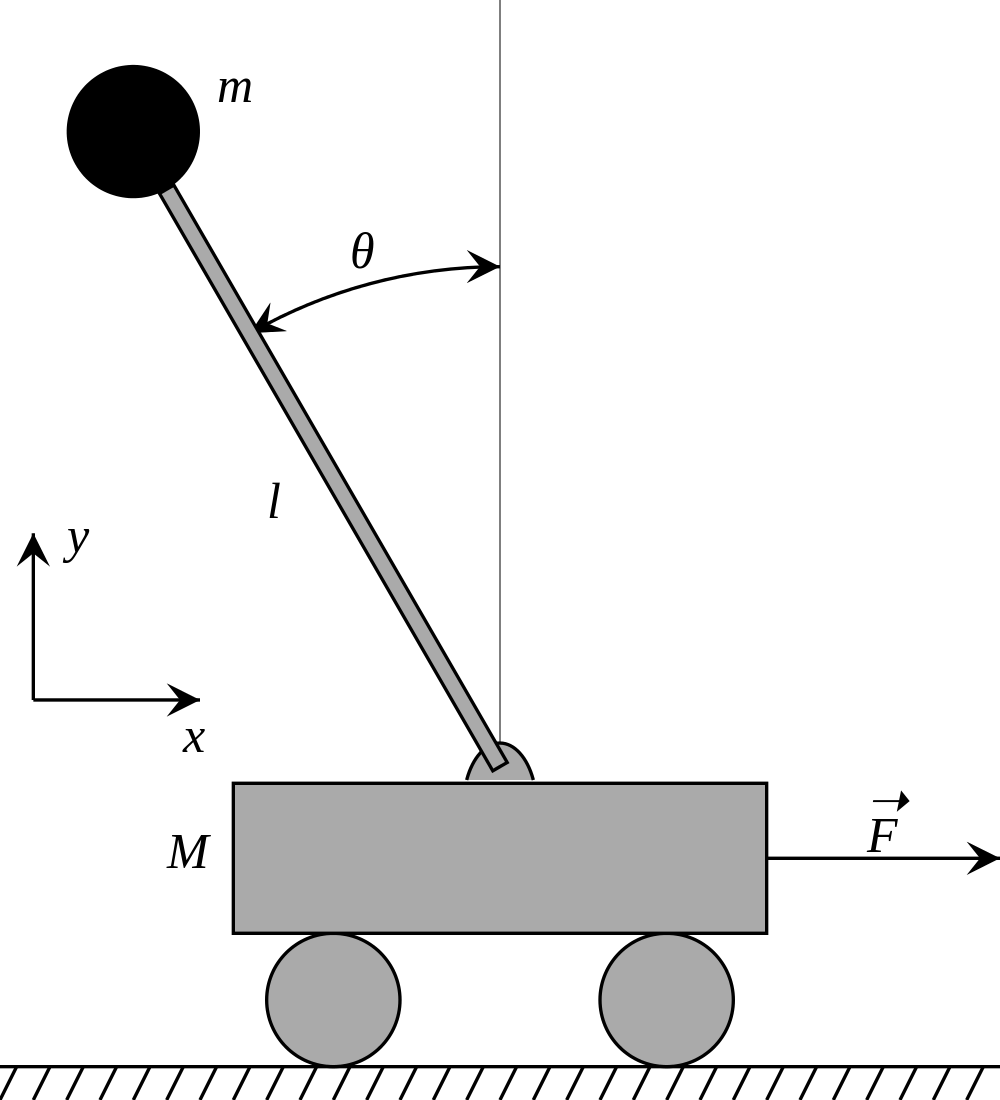
\includegraphics[width=\linewidth]{images/cart-pole.png}
    \label{fig:enter-label}
  \end{figure}

  \end{minipage}\qquad\quad
  \begin{minipage}[t]{0.5\linewidth}

    \vspace{3em}

    Goal: keep the stick up

    \begin{itemize}
    \item state: angle of the stick
    \item reward: $1$ if still up, $0$ otherwise
    \end{itemize}

    \vspace{1em}

    Idea: run episodes of length $H = 250$

    $\rightarrow$ adapt policy after each episode

  \end{minipage}
  
\end{frame}


\begin{frame}{Example: CartPole}
  Cumulative reward, 1 vs. 10 carts

  \vspace{-1em}
  
  \begin{figure}
    \centering
    \resizebox{!}{9em}{
    \begin{tikzpicture}
      \node at (0, 0)  {~};
      \node at (0, 2)  {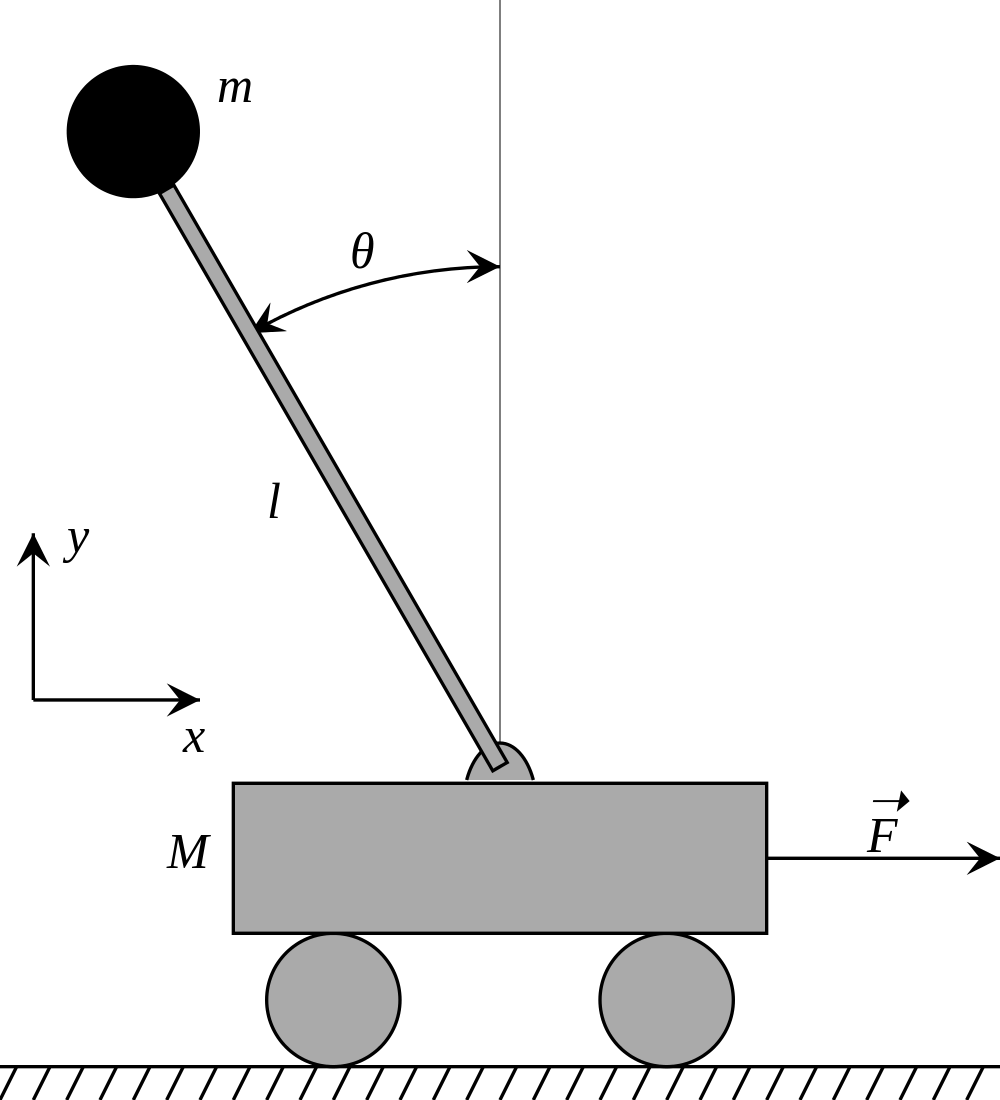
\includegraphics[width=0.05\linewidth]{images/cart-pole.png}};
      \node at (0, 4)  {~};
    \end{tikzpicture}}
    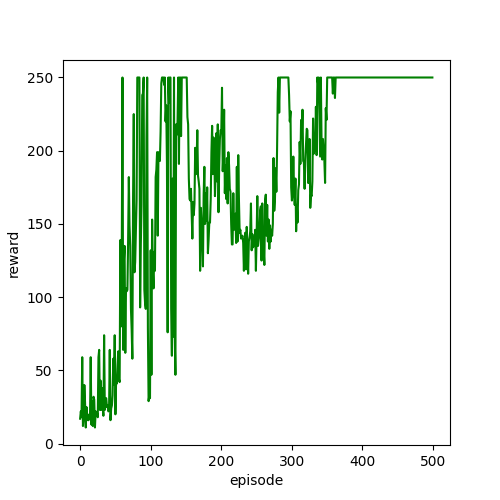
\includegraphics[width=0.35\linewidth]{images/CartPole1.png}
    \qquad
    \resizebox{!}{9em}{
    \begin{tikzpicture}
      \node at (0, 0)  {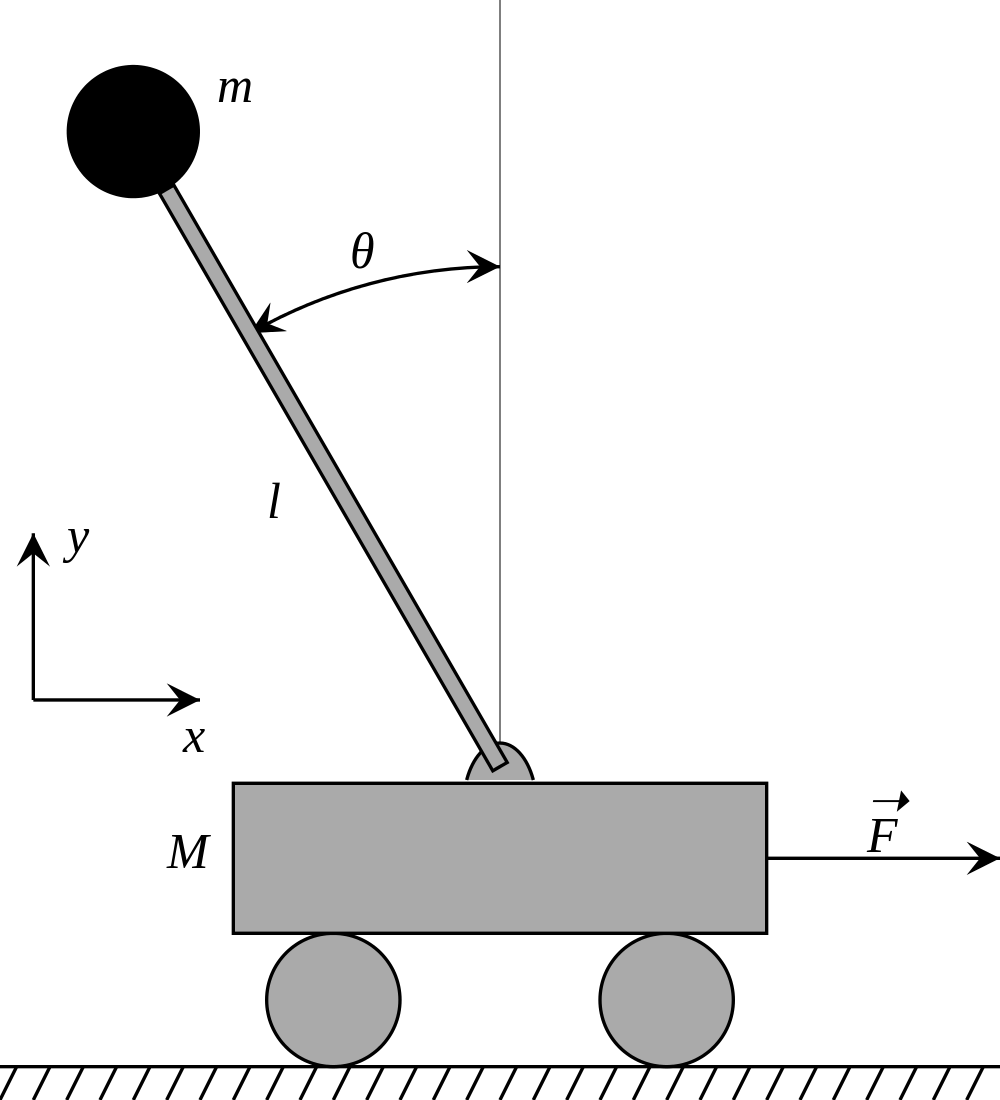
\includegraphics[width=0.05\linewidth]{images/cart-pole.png}};
      \node at (0, 1)  {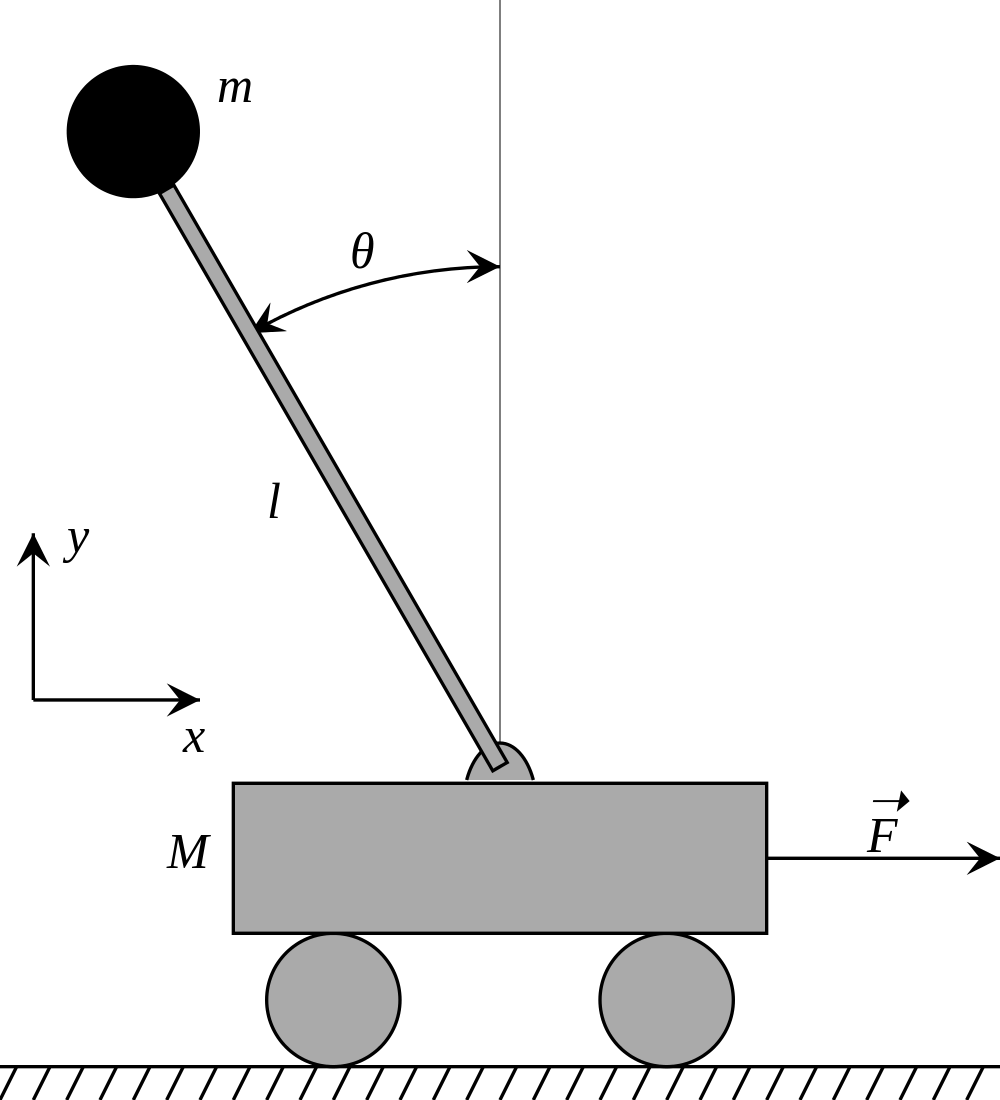
\includegraphics[width=0.05\linewidth]{images/cart-pole.png}};
      \node at (0, 2)  {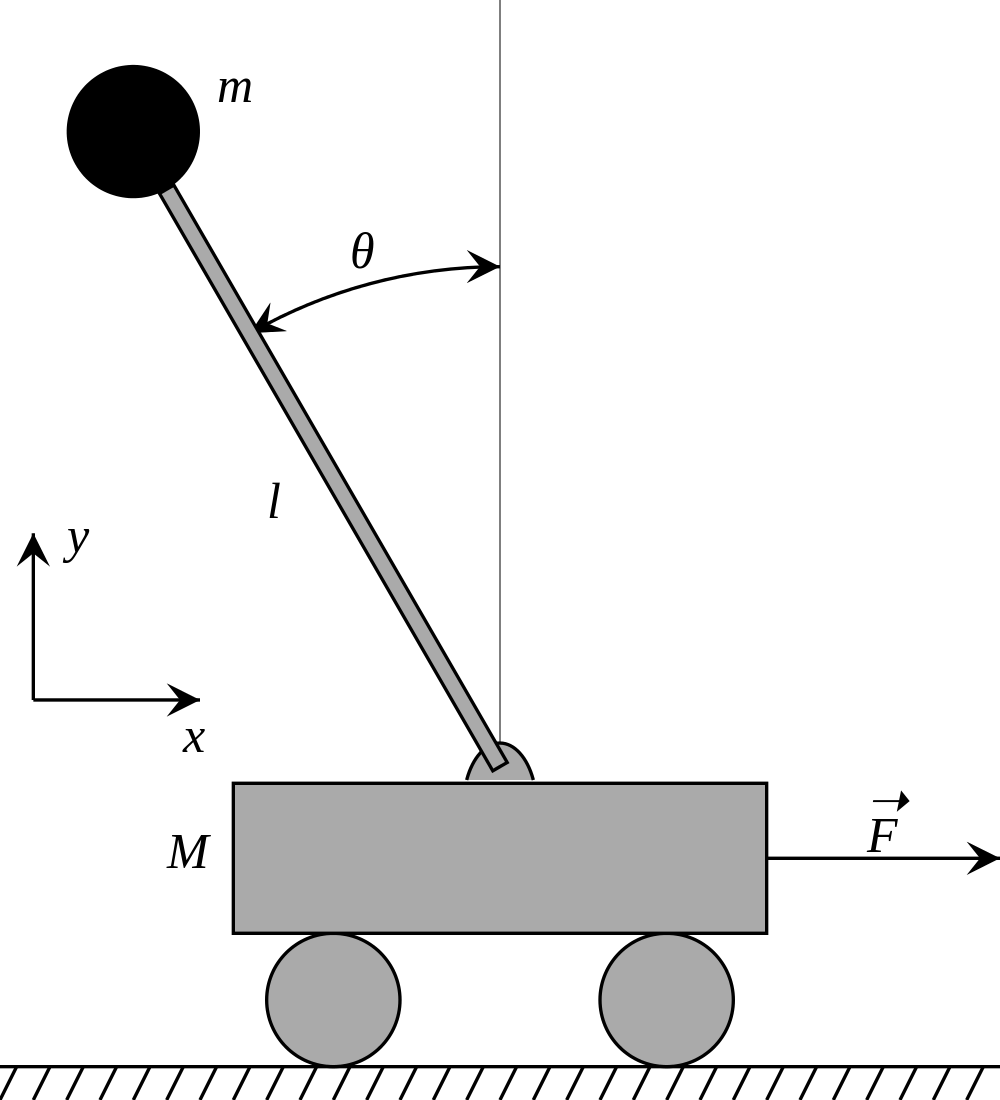
\includegraphics[width=0.05\linewidth]{images/cart-pole.png}};
      \node at (0, 3)  {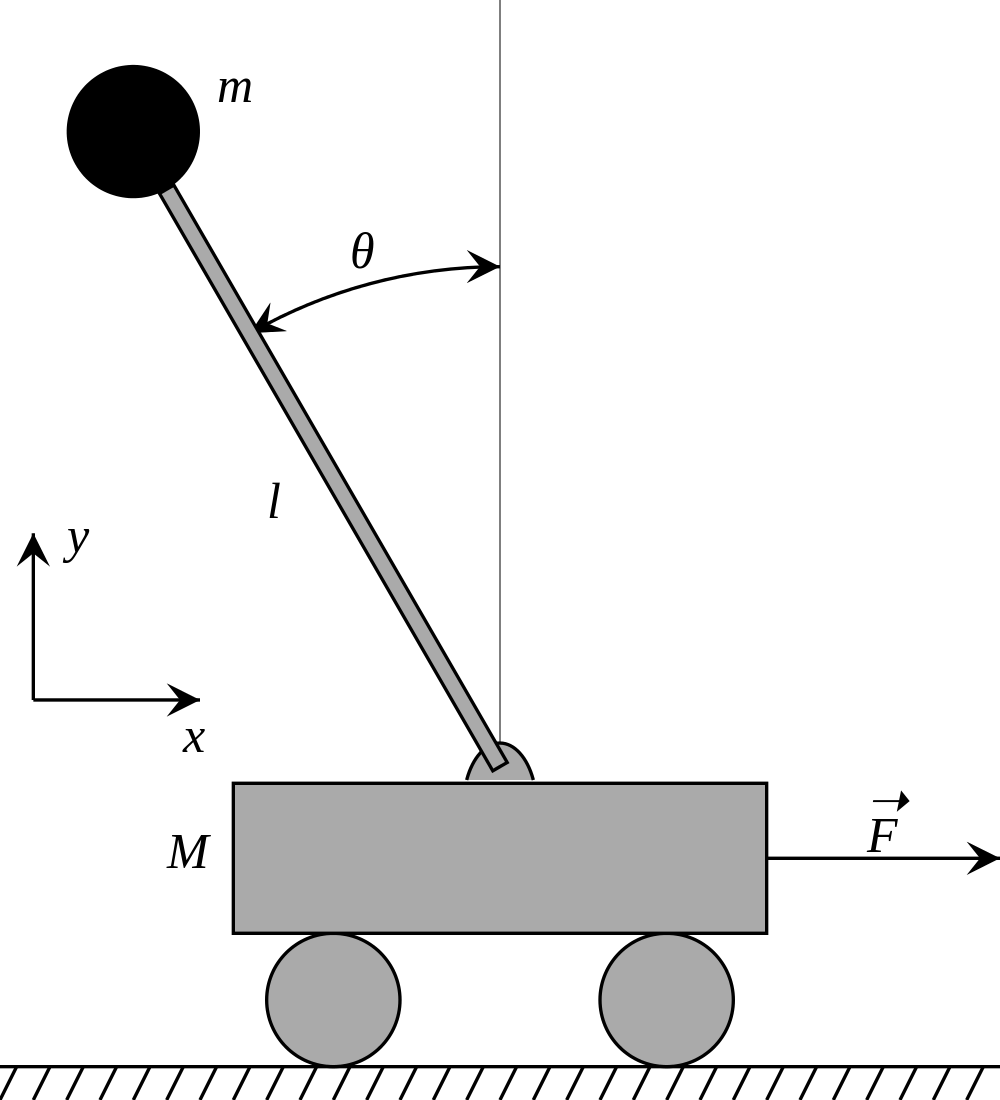
\includegraphics[width=0.05\linewidth]{images/cart-pole.png}};
      \node at (0, 4)  {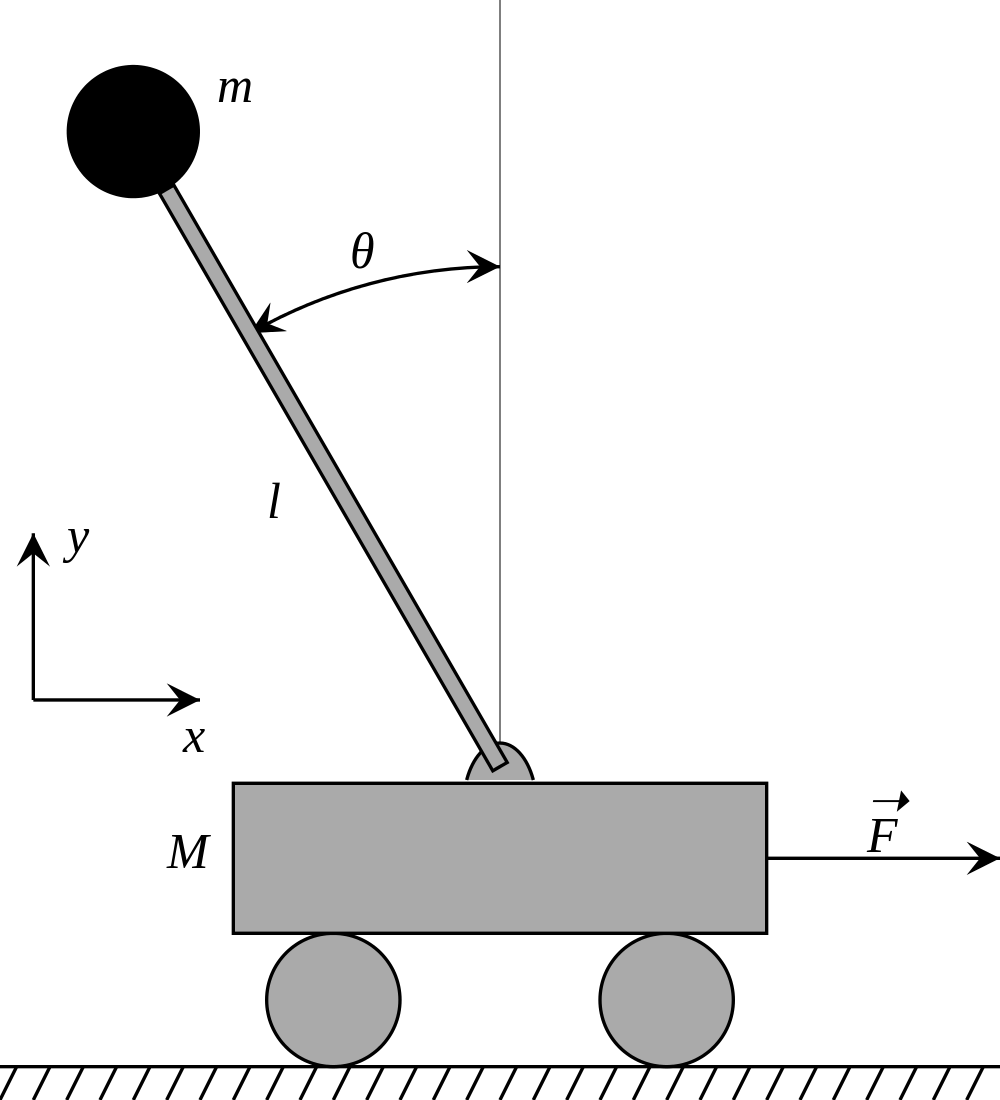
\includegraphics[width=0.05\linewidth]{images/cart-pole.png}};
      \node at (1, 0)  {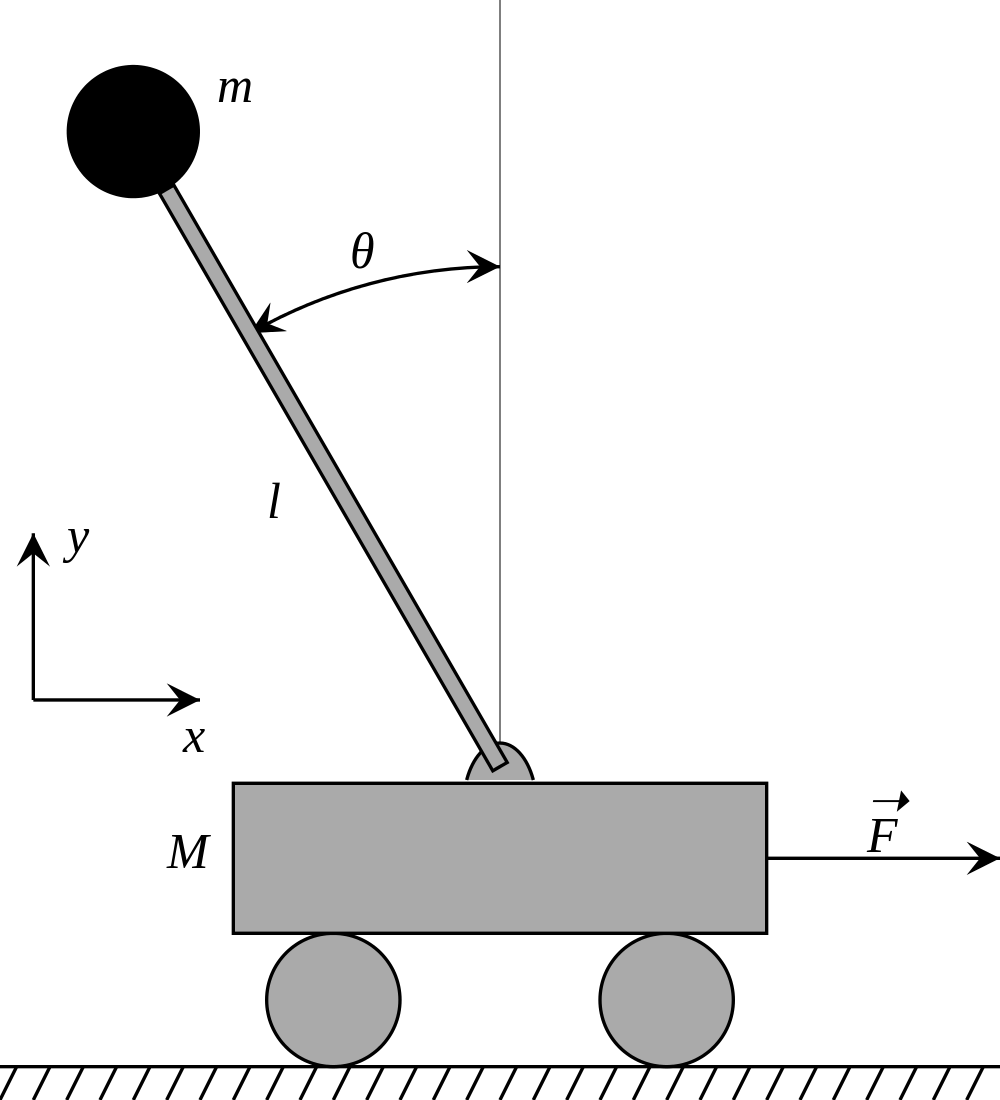
\includegraphics[width=0.05\linewidth]{images/cart-pole.png}};
      \node at (1, 1)  {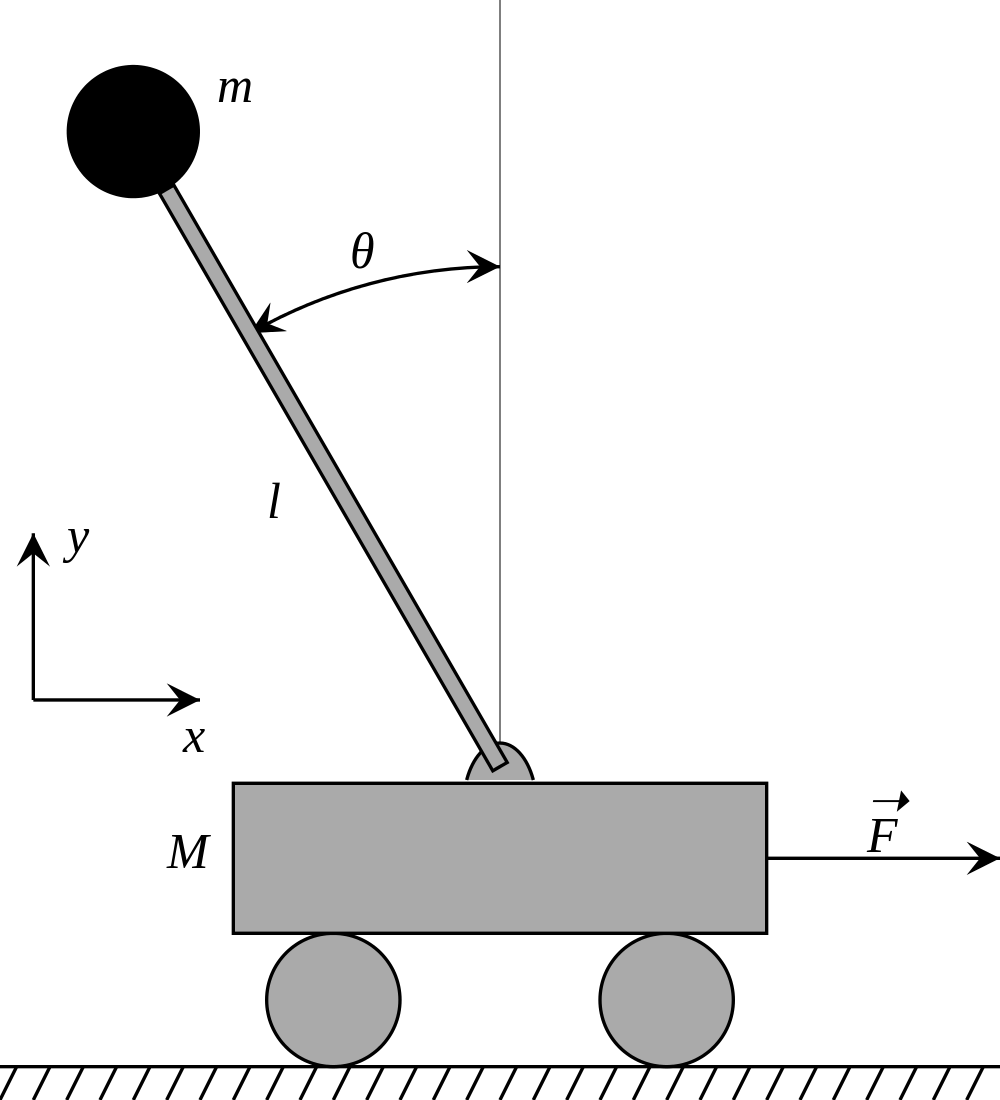
\includegraphics[width=0.05\linewidth]{images/cart-pole.png}};
      \node at (1, 2)  {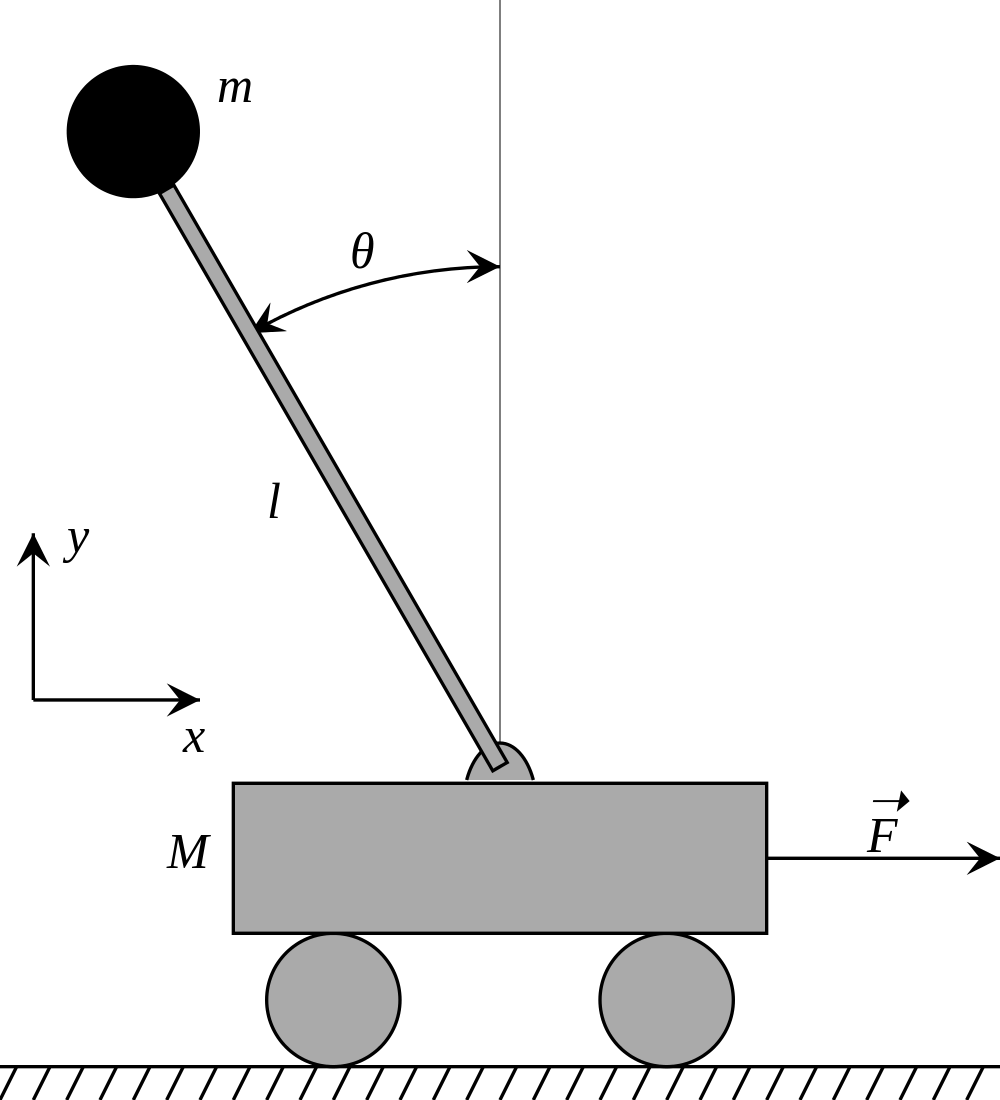
\includegraphics[width=0.05\linewidth]{images/cart-pole.png}};
      \node at (1, 3)  {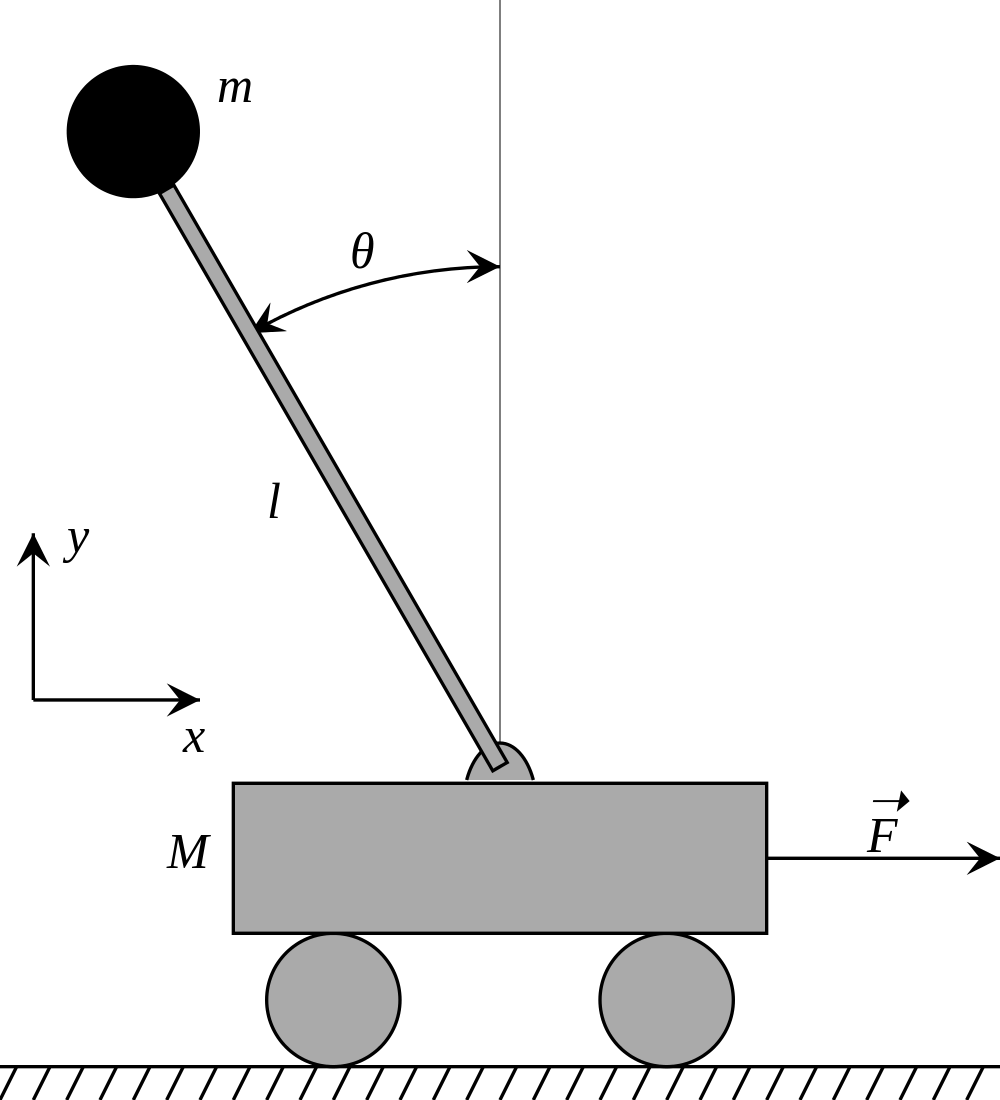
\includegraphics[width=0.05\linewidth]{images/cart-pole.png}};
      \node at (1, 4)  {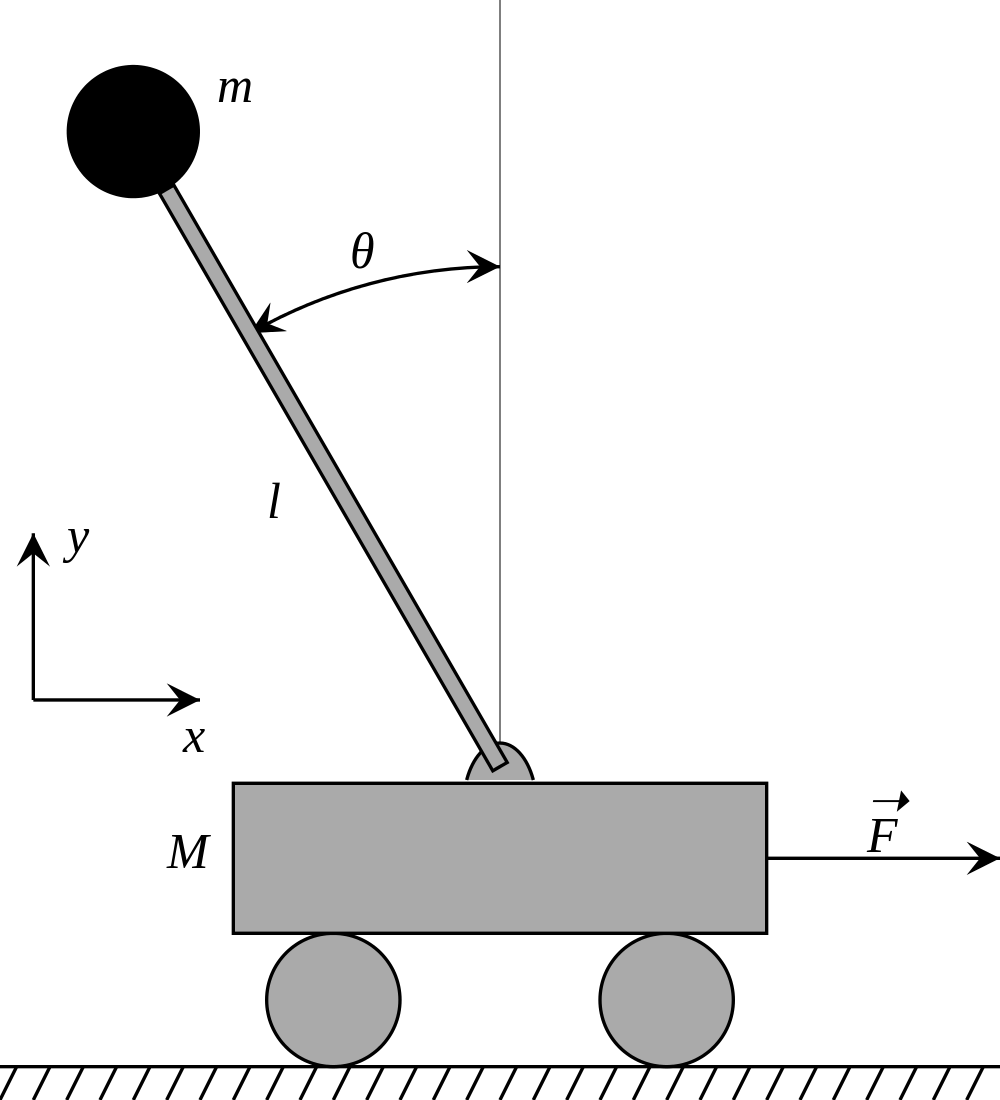
\includegraphics[width=0.05\linewidth]{images/cart-pole.png}};
    \end{tikzpicture}}
    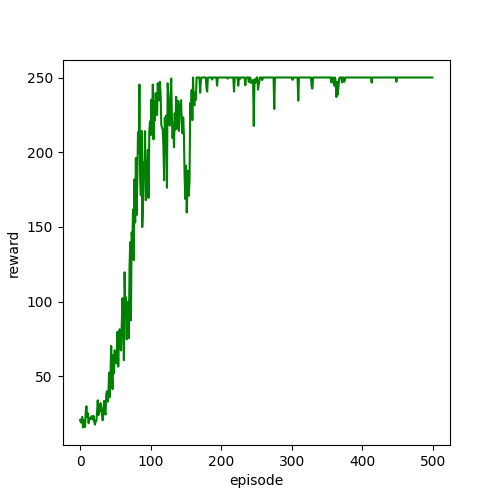
\includegraphics[width=0.35\linewidth]{images/CartPole10.png}
    \label{fig:enter-label}
  \end{figure}

\end{frame}




\begin{frame}
  \begin{center}
    \textcolor{beamer@blendedblue}{
      \huge Federated \\[1em]
      \huge Reinforcement Learning in V2X
    }
  \end{center}

  \vspace{2em}

  Based on \fullcite{mancini2024joint}
\end{frame}

\begin{frame}{Vehicle-to-Everything Communication}
  \begin{center}
    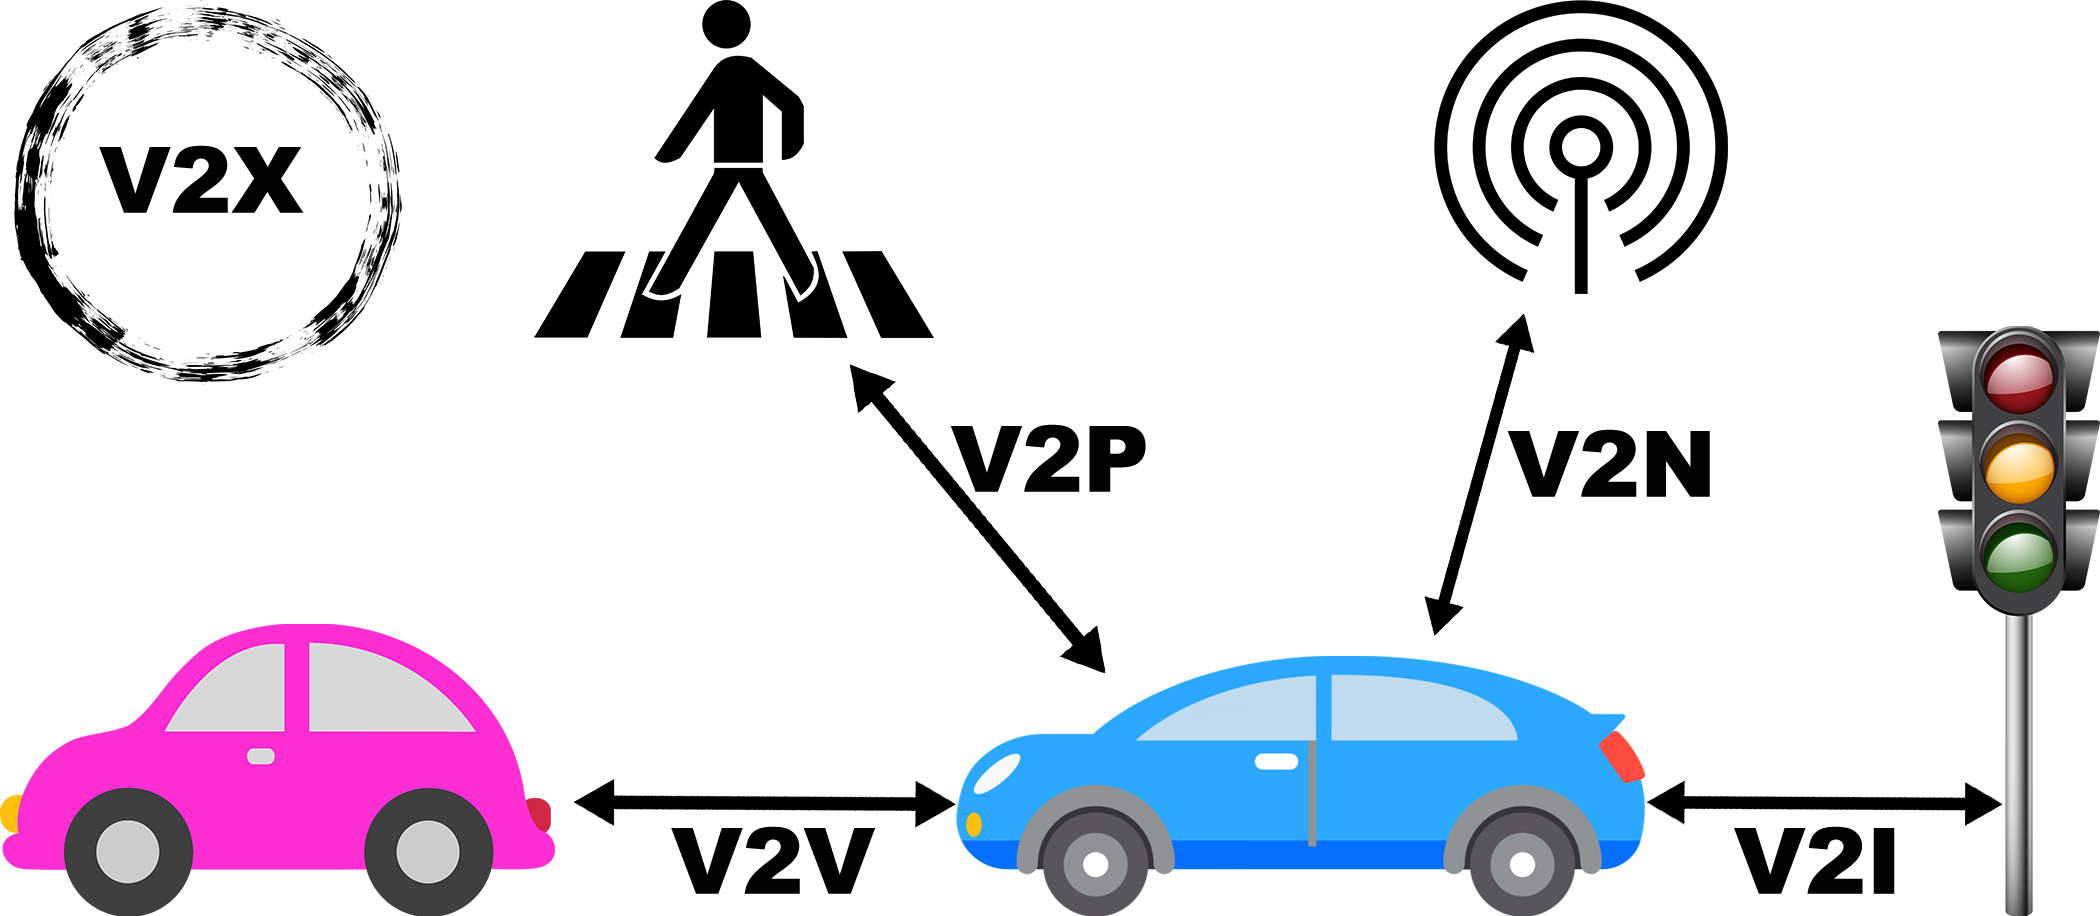
\includegraphics[width=0.7\linewidth]{images/Types_V2X.png}
  \end{center}
  
\end{frame}


\begin{frame}[fragile]{Reinforcement Learning for V2X}
  \vspace{-1em}

  Scenario:

  \vspace{-0.5em}
  
  \begin{itemize}
  \item Two vehicles on a road, each vehicle is a \textbf{RL agent}  
  \item \textbf{Task:} choose combination of channels for communication\footfullcite{serpentine}
    \begin{itemize}
    \item \textcolor{beamer@blendedblue}{ \bfseries Visible Light (VLC) }: front and tail light, directional (``cheap'')
    \item \textcolor{beamer@blendedblue}{ \bfseries DSRC }: all-around communication, any direction (``expensive'')
    \end{itemize}
  \end{itemize}

  \vspace{-1em}

        
  \begin{figure}
    \centering
    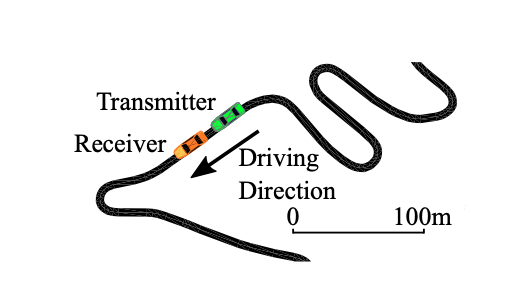
\includegraphics[scale=0.3]{images/vehicles.png}
  \end{figure}

  
  \vspace{1em}

\end{frame}


\begin{frame}[fragile]{Federated Reinforcement Learning for V2X}
  Scenario:
  \begin{itemize}
  \item Many vehicles on \textcolor{beamer@blendedblue}{\textbf{different roads}}, pairwise interactions between vehicles\footfullcite{flexe}
  \end{itemize}

  \vspace{-1.5em}
        
  \begin{figure}
    \centering
    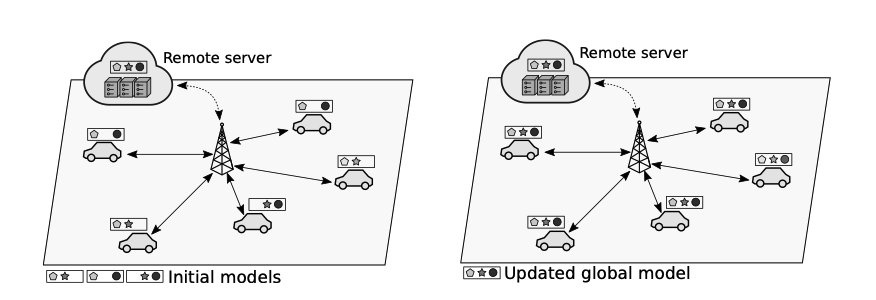
\includegraphics[scale=0.4]{images/grid.png}
  \end{figure}

  
  \vspace{0.5em}

\end{frame}

\begin{frame}{Federated Actor-Critic\footfullcite{qi2021federated}}
  Use two deep neural networks:
  \begin{itemize}
  \item \textcolor{beamer@blendedblue}{\textbf{actor}}: function that determines the way actions are choosen (``policy'')
  \item \textcolor{beamer@blendedblue}{\textbf{critic}}: function that estimates the value function
  \end{itemize}

  In federated actor critic methods, agents:
  \begin{itemize}
  \item collect local data by interacting with their environment
  \item update their local actor and critic
  \end{itemize}

  $\rightarrow$ after a number of updates, local actor and critic are aggregated!

  \vspace{1.5em}
\end{frame}

\begin{frame}{Experimental Setup}
  \begin{itemize}
  \item 
    Different roads: countryside, highway and urban
    \begin{center}
      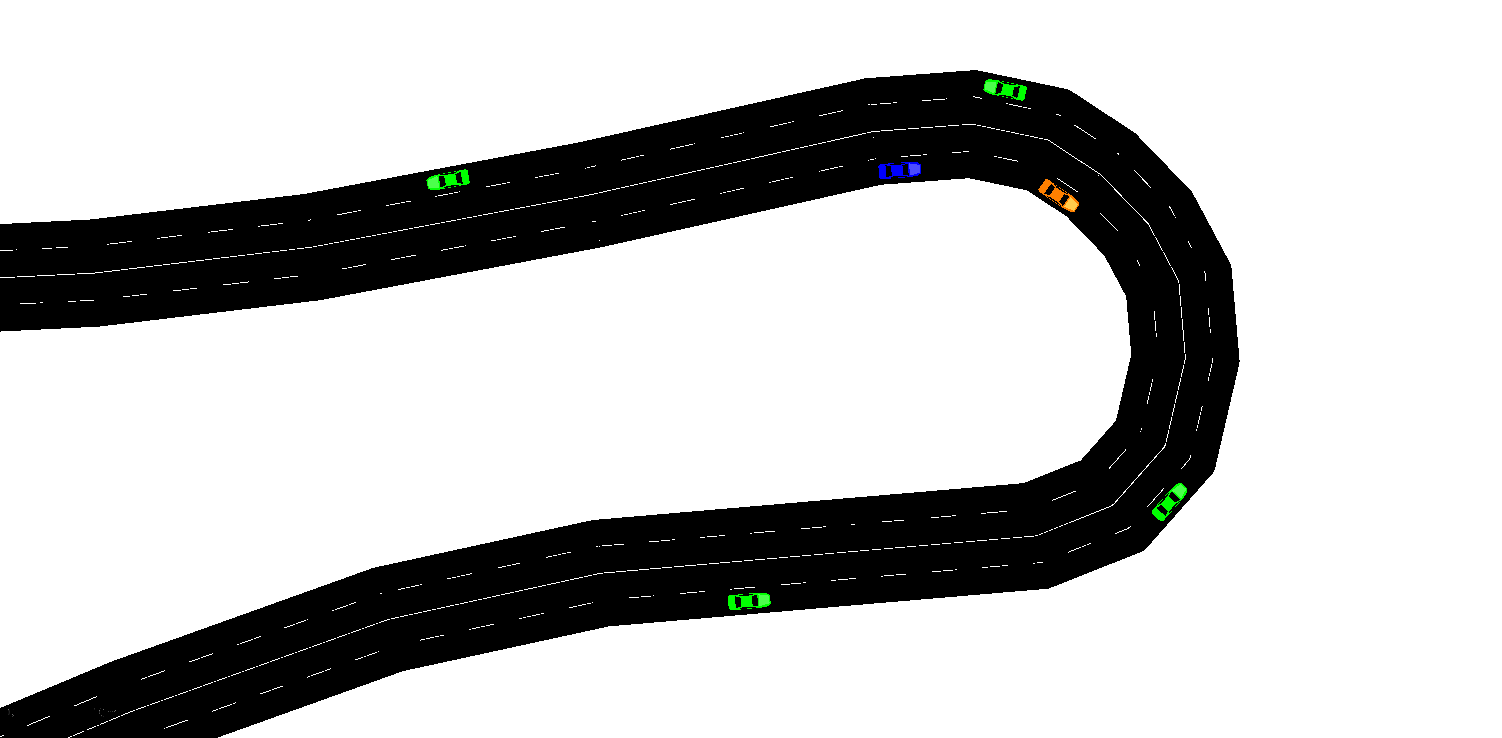
\includegraphics[width=0.2\linewidth]{images/countryside.png}
      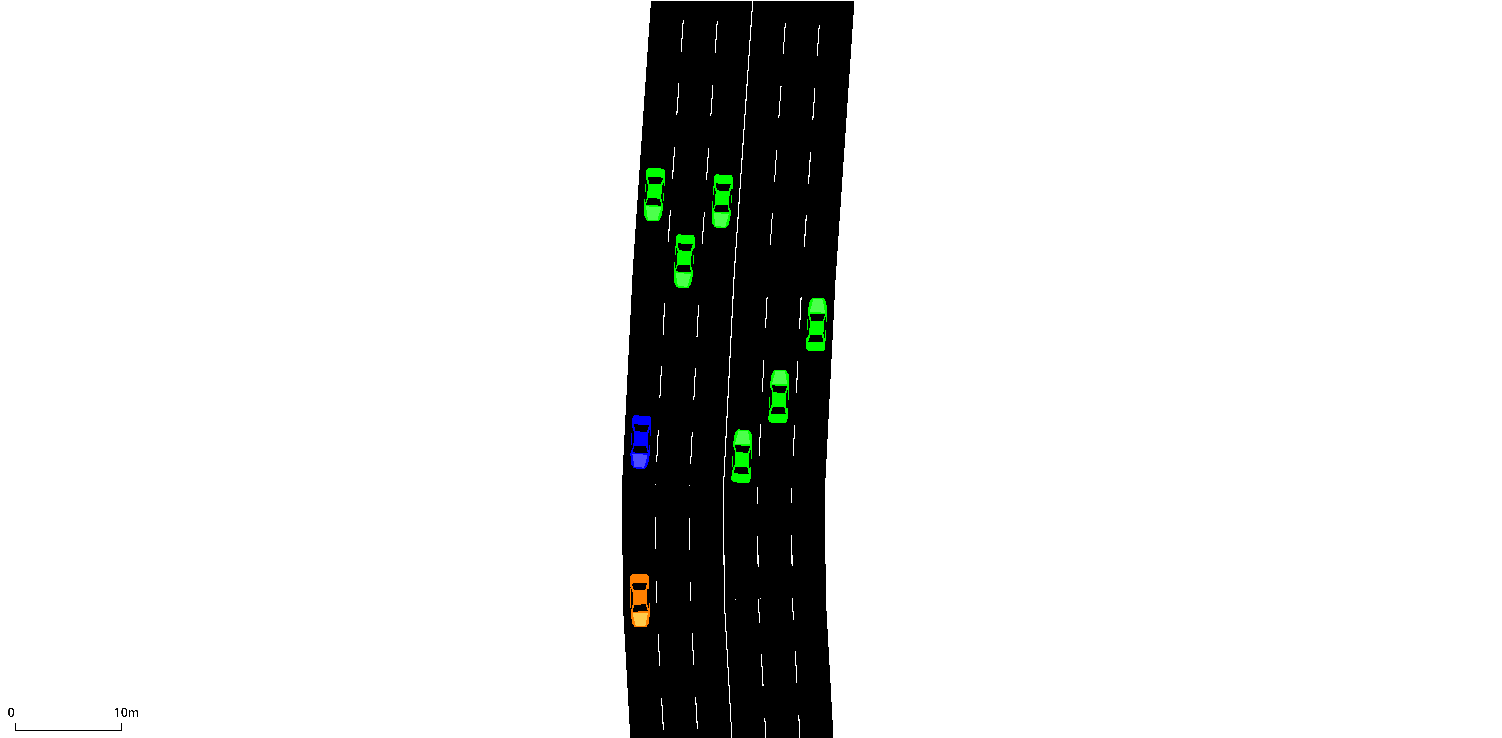
\includegraphics[width=0.2\linewidth]{images/highway.png}
      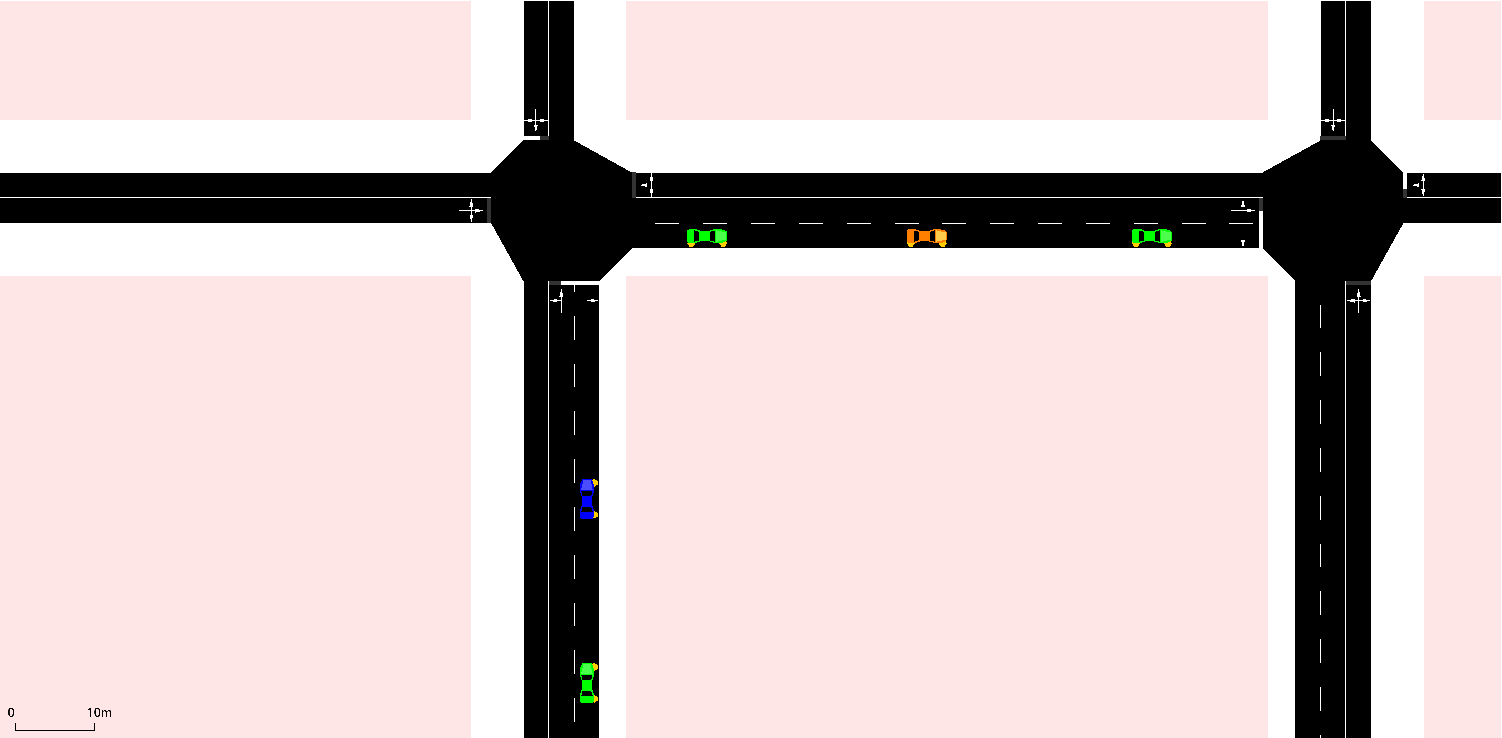
\includegraphics[width=0.2\linewidth]{images/grid_road.png}
    \end{center}

    \vspace{0.5em}
    
  \item Different road occupation:
    \begin{center}
      \resizebox{!}{2em}{
        \begin{tabular*}{\textwidth}{@{\extracolsep{\fill}} cccc }
          \toprule
          & 
            \textbf{Countryside}  &  \textbf{Highway} & \textbf{Urban}\\
          \midrule
          Speed of vehicles (m/s) & $\sim 20 $ &  $\sim 30 $ & $\sim 15 $ \\
          Speed of bg. vehicles (m/s) & $25-35$ & $35-45$ & $20-25$\\
          Background traffic density  & $0-50$ & $0-50$ & $0-50$\\
          \bottomrule
        \end{tabular*}
      }
    \end{center}

    \vspace{0.5em}

  \item Different antennas:
  \begin{center}
    \textit{monopole}, \textit{panorama} or \textit{patch}
  \end{center}
  \end{itemize}
\end{frame}



\begin{frame}{Results: Cumulative Rewards}
  Take $30$ agents, training on only part of the roads:

  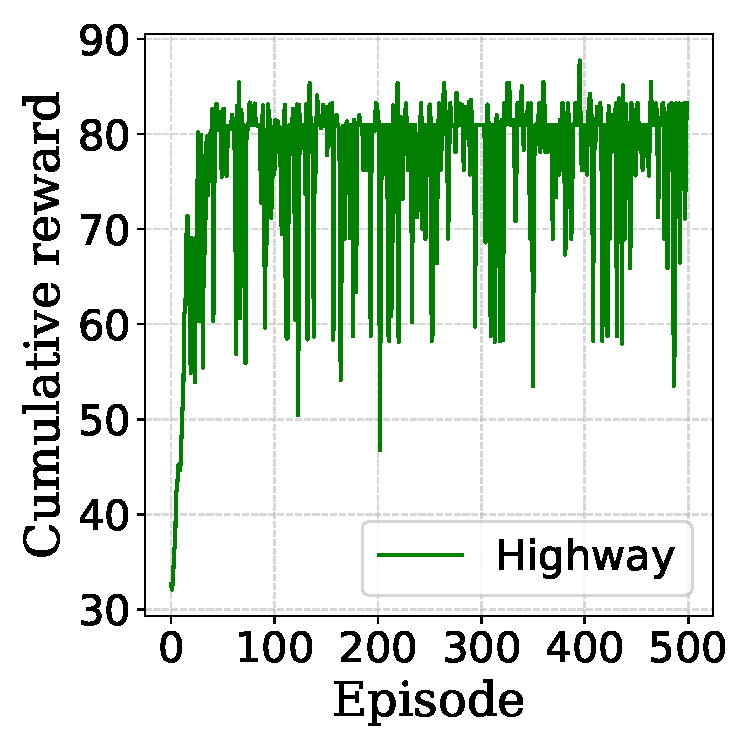
\includegraphics[width = 0.24\textwidth]{images/baseline_highway.pdf}
  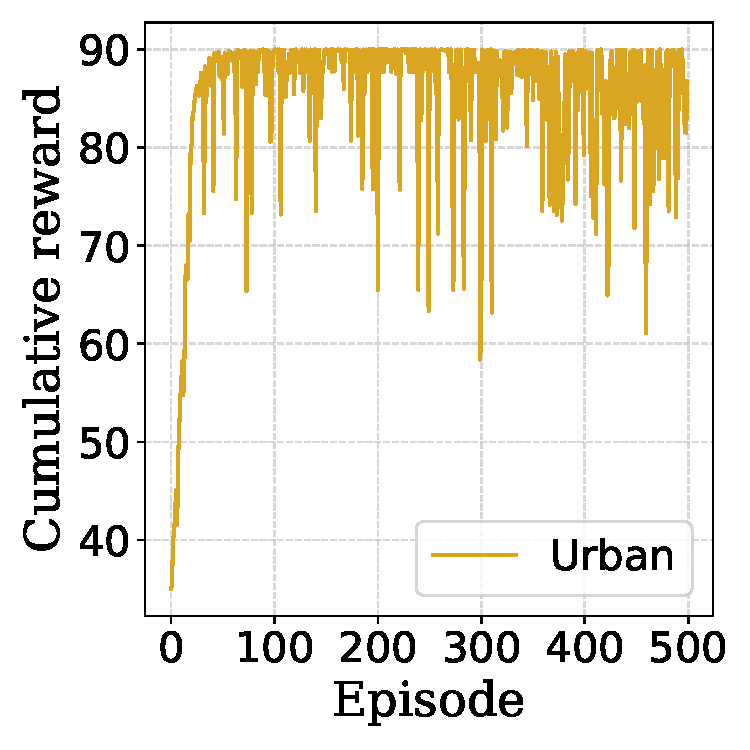
\includegraphics[width = 0.24\textwidth]{images/baseline_urban.pdf}
  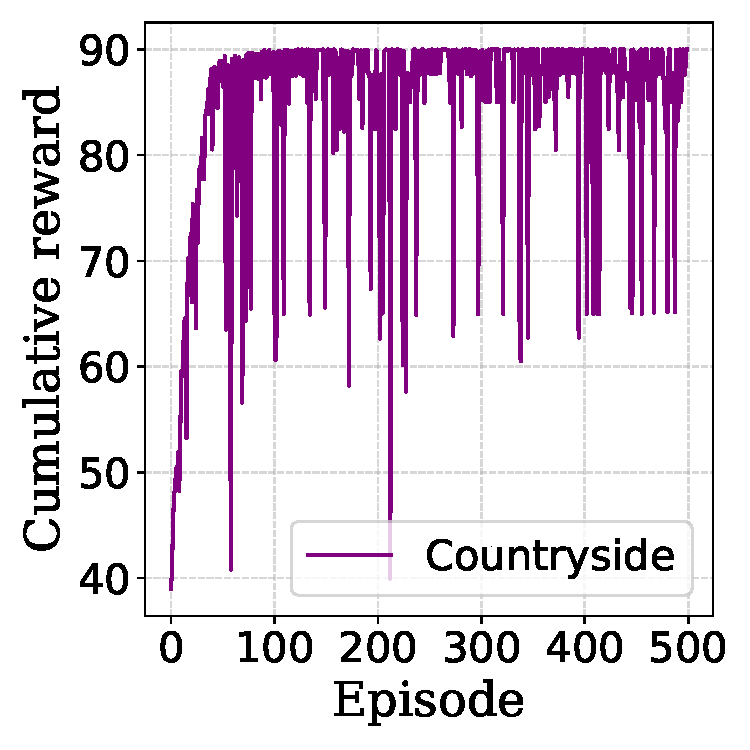
\includegraphics[width = 0.24\textwidth]{images/baseline_ctr.pdf}
  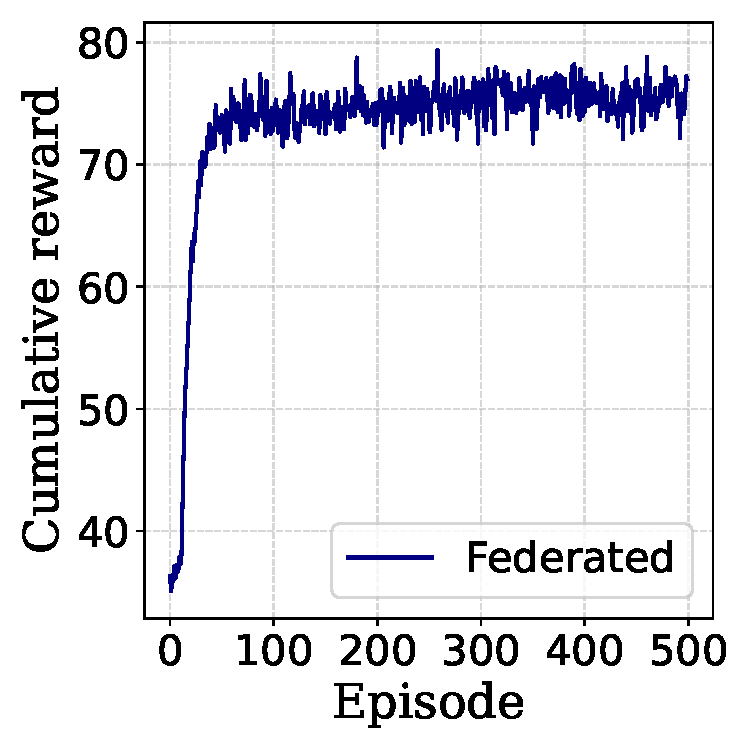
\includegraphics[width = 0.24\textwidth]{images/learning_curve_federated_new.pdf}  
\end{frame}

\begin{frame}{Results: Reliability}
  Ratio of messages received on a test scenario:
  \begin{table}[t]
    \centering
    \begin{tabular*}{\textwidth}{@{\extracolsep{\fill}} ccccc }
      \toprule
      \textbf{} & \textbf{Urban} & \textbf{Country} & \textbf{Highway} & \textbf{All} \\
      \midrule
      Trained on urban & $0.656$ & $0.738$ & $0.862$ & $0.752$ \\
      Trained on country & $0.654$ & $0.784$ & $0.974$ & $0.804$  \\
      Trained on highway & $0.655$ & $0.740$ & $\mathbf{0.975}$ &  $0.790$\\
      Trained on all (federated) & $\mathbf{0.724}$ & $\mathbf{0.923}$ & $0.974$ & $\mathbf{0.874}$ \\
      \bottomrule
    \end{tabular*}
  \end{table}


  \textcolor{beamer@blendedblue}{
    $\rightarrow$ federated RL learns more reliable policies!
  }
\end{frame}

\begin{frame}{Summary for Federated V2X}
  \begin{itemize}
  \item Federated PPO works in V2X
  \item It learns more reliable policies
  \item The learning process is less noisy
  \end{itemize}
\end{frame}

\begin{frame}
  \begin{center}
    \textcolor{beamer@blendedblue}{
      \huge Federated \\[1em]
      \huge Temporal Difference Learning
    }
  \end{center}

  \vspace{2em}

  Based on \fullcite{mangold2024scafflsa}
\end{frame}




\begin{frame}{Federated TD Learning\footfullcite{sutton2018}${}^,$\footfullcite{wang2024federated} }
  In Federated TD, $N$ agent use a shared policy $\pi$ in $N$ different environments:
  \begin{align*}
    S_0^c= s, 
    A_k^c \sim \pi(\cdot | S_k^c), 
    \text{ and }
    S_{k+1}^c \sim P^c_{\text{MDP}}(\cdot| S_k^c,A_k^c)
  \end{align*}

  \pause
  
  Goal: estimate its value in each environment, for $s \in \mathcal{S}$,
  \begin{align*}
    V^{c,\pi}(s) = \textstyle{\mathbb{E}\left[\sum_{k=0}^{\infty}\gamma^{k} r^{c}(S_k^c,A_k^c)\right]}
  \end{align*}
  where $\gamma < 1$ is the discount factor, and $r^c$ is a reward obtained by agent $c$

  \vspace{2em}
  
\end{frame}


\begin{frame}{ TD Learning with linear approximation}

  Idea: build a \emph{shared estimate} of all values
  \begin{align*}
    V^{c,\pi}(s) \approx \theta^\top \varphi(s)
  \end{align*}
  using $\theta \in \mathbb{R}^d$ and embedding $\varphi: \mathcal{S} \rightarrow \mathbb{R}^d$

  \vspace{1em}
  
  \pause

  Is this meaningful to use a shared estimate? Yes, because:
  \begin{itemize}
  \item If agents are homogeneous, it reduces sample complexity
  \item If agents are heterogeneous, it may reduce bias of local data
  \end{itemize}
\end{frame}



\begin{frame}{Federated TD Algorithm}
  Similarly to Federated Averaging:

  \vspace{-0.5em}
  
  \begin{itemize}
  \item For each $t = 0 ...$ :
    \begin{itemize}
      \normalsize
    \item Set $\theta_{t,0}^c = \theta_t$
    \item For each agent $c$, do $K$ local updates: \\[0.5em]
      Choose action $a_{t,k} \sim \pi(\cdot | s_{t,k})$

      Receive reward $r_{t,k}$, new state $s_{t,k+1}$ and perform local update:
      
      \begin{center}
        ~~~~~~$\theta_{t,k} = \theta_{t,k-1}^c - \eta \times \text{TD\_Error}(s_{t,k}, r_{t,k}, a_{t,k}, s_{t,k+1})$
      \end{center}
      
      \vspace{0.5em}
      
    \end{itemize}
  \item Aggregate local updates $\theta_{t+1} = \tfrac{1}{N} \sum\nolimits_{c=1}^{N} \theta_{t,K}^c $
  \end{itemize}

  \vspace{1.5em}  
\end{frame}
\begin{frame}{Analysis of Federated TD}

  We proved convergence rate:
  \begin{align*}
    \mathbb{E} \Big[ \| {\theta_t - \textcolor{beamer@blendedblue}{\mathbf{\theta^{bias}_{\infty}}} - \theta_\star} \|^2 \Big]
    =
    O\left(
    (1 - \eta a)^{K t} \| \theta_0 - \theta_\star \|^2
    + \frac{\eta \sigma_\star^2}{N a}
    \right)
  \end{align*}

  For some $\theta_\infty^{\text{bias}} \in \mathbb{R}^d$, $a > 0$, $\sigma_\star^2 \ge 0$

  \pause

  \vspace{1em}

  \small \color{gray} We can characterize the bias of FedLSA:
  \begin{align*}
    \theta_\infty^{\text{bias}}
    & =
      \frac{1}{N}
      \sum_{c=1}^N
      (\text{Id} - (\text{Id}- \eta A)^K)^{-1} 
      (\text{Id} - (\text{Id}- \eta A^c)^K)\{ \theta_\star^c - \theta_\star \}
  \end{align*}


\end{frame}



\begin{frame}{Numerical Illustration}
  \vspace{-0.5em}
  
  \begin{center}
    ~~~~~Left: K=100~~~~~~~~~~~~~~~~~~~~~
    Right: K=1000
 
    \vspace{-1em}
   
    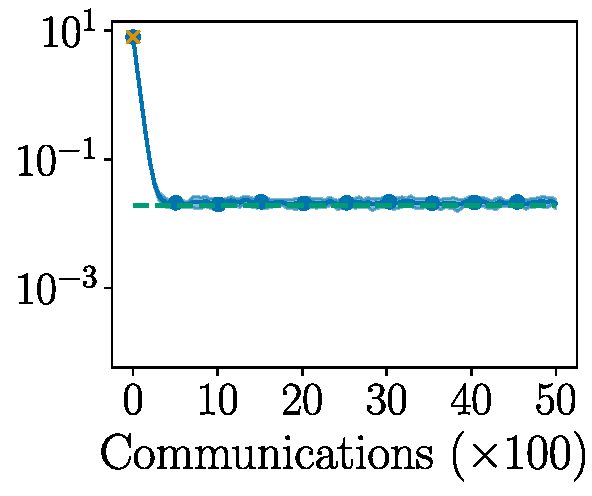
\includegraphics[width=0.4\linewidth]{images/plot_hg_100_n100_fedlsa.pdf}
    ~~
    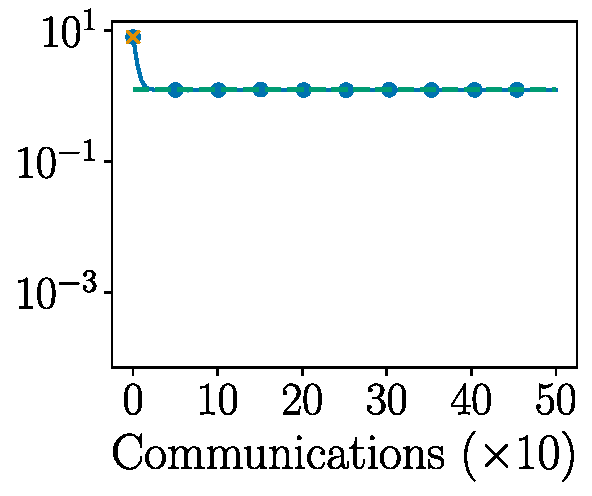
\includegraphics[width=0.4\linewidth]{images/plot_hg_1000_n100_fedlsa.pdf}
  \end{center}

  \vspace{-1em}

  Blue line: FedLSA's mean squared error

  \vspace{-1em}

  Green line: FedLSA's bias as predicted by our theory


  \only<2>{%
    \tikz[overlay,remember picture]
    \node[fill=beamer@blendedblue!10,text=black,inner sep=2em,line width=2pt,draw=beamer@blendedblue] at ([xshift=0cm,yshift=0cm]current page.center){\Large Problem: heterogeneity requires many communications};
  }  
\end{frame}


\begin{frame}{Solution: Control variates (SCAFFLSA)\footnote{Extending ideas from on \fullcite{karimireddy2020scaffold}}}
  Similarly to Federated Averaging:

  \vspace{-0.5em}
  
  \begin{itemize}
  \item For each $t = 0 ...$ :
    \begin{itemize}
      \normalsize
    \item Set $\theta_{t,0}^c = \theta_t$
    \item For each agent $c$, do $K$ local updates: \\[0.5em]
      Choose action $a_{t,k} \sim \pi(\cdot | s_{t,k})$

      Receive reward $r_{t,k}$, new state $s_{t,k+1}$ and perform local update:
      
      \begin{center}
        ~~~~~~$\theta_{t,k} = \theta_{t,k-1}^c - \eta \times \Big\{ \text{TD\_Error}(s_{t,k}, r_{t,k}, a_{t,k}, s_{t,k+1}) + \textcolor{beamer@blendedblue}{\mathbf{\xi_t^c}} \Big\}$ 
      \end{center}
      
      \vspace{0.5em}
      
    \end{itemize}
  \item Aggregate local updates $\theta_{t+1} = \tfrac{1}{N} \sum\nolimits_{c=1}^{N} \theta_{t,K}^c $
  \item \textcolor{beamer@blendedblue}{\bfseries Update control variate $\mathbf{\xi_{t+1}^c = \xi_t^c + \frac{1}{\eta K} ( \theta_{t,K}^c - \theta_{t+1})}$}
  \end{itemize}

  \vspace{1em}  
\end{frame}


\begin{frame}{Convergence Rate}
  We prove, assuming $K \le \frac{a}{\eta \max_c \| A^c \|^2}$
  \begin{align*}
    \mathbb{E}[\| \theta_{T} - \theta_\star \|^2]
    & \lesssim{}
      \big( 
      1 - \tfrac{\eta a K}{2}
      \big)^T \psi_0
      +
      \frac{\eta \sigma_\star^2}{N a}
  \end{align*}
  with $\psi_0 = \| \theta_0 - \theta_\star \|^2 + \eta^2K^2 \mathbb{E}_c[\| A^c( \theta_\star^c - \theta_\star) \|^2]$
\end{frame}



\begin{frame}{Numerical Illustration}
  \vspace{-0.5em}
  
  \begin{center}
    ~~~~~Left: K=100~~~~~~~~~~~~~~~~~~~~~
    Right: K=1000
 
    \vspace{-1em}
   
    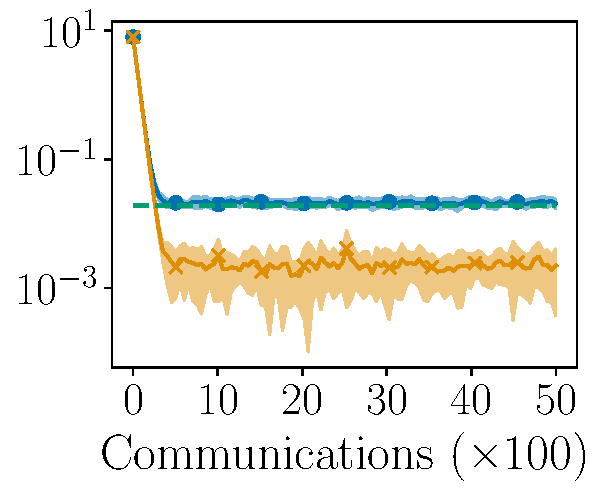
\includegraphics[width=0.4\linewidth]{images/plot_hg_100_n100.pdf}
    ~~
    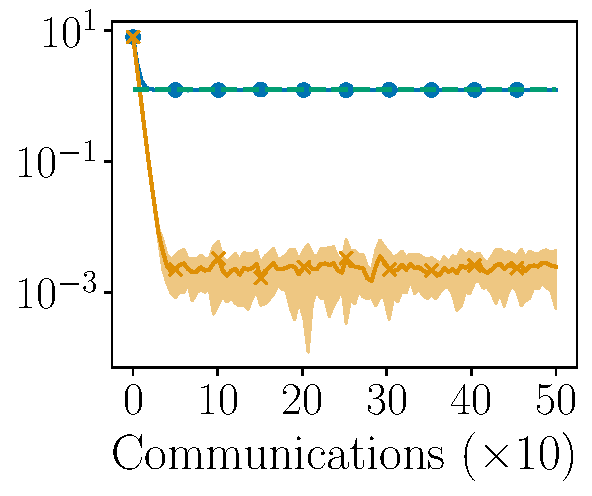
\includegraphics[width=0.4\linewidth]{images/plot_hg_1000_n100.pdf}
  \end{center}

  \vspace{-1em}

  Blue line: FedLSA's mean squared error

  \vspace{-1em}

  Orange line: SCAFFLSA's mean squared error
\end{frame}


\begin{frame}{Summary for Federated TD}
  \begin{itemize}
  \item Analysis of TD learning with exact characterization of bias
  \item Control variate method for TD learning works
  \item We have linear speed-up!
  \end{itemize}
\end{frame}

  
%\begin{frame}{Focus: linear speed-up}
  
%\end{frame}


\begin{frame}
  \begin{center}
    \textcolor{beamer@blendedblue}{
      \huge Federated \\[1em]
      \huge Value Iteration
    }
  \end{center}

  \vspace{2em}

  Based on \fullcite{labbi2024federated}

\end{frame}

\begin{frame}{State-Value Functions}
  Finite-horizon value function/reward to-go:
  \begin{align*}
    \nonumber 
    V_h^{(\pi)}(s) = \mathbb{E}\left[ {\sum_{h'=h}^{H}r_h(s_{h'},a_{h'})} ~\bigg|~ {s_{h}=s}\right]
  \end{align*}

  Value when starting with action $a$:
  \begin{align*}
    Q_h^{(\pi)}(s,a) := \mathbb{E}\left[ {\sum_{h'=h}^{H} {r_{h'}}(s_{h'},a_{h'})} ~\bigg|~ {s_{h}=s, a_{h}=a}
    \right]
  \end{align*}

  \pause

  $\rightarrow$ Crucial idea of RL: take action $a = \argmax_{a \in A} Q_1^{\pi}(s, a)$ to improve policy

  \only<3>{%
    \tikz[overlay,remember picture]
    \node[fill=beamer@blendedblue!10,text=black,inner sep=2em,line width=2pt,draw=beamer@blendedblue] at ([xshift=0cm,yshift=0cm]current page.center){\Large Goal: learn the best policy!};
  }  

\end{frame}

\begin{frame}{From Value to Bellman}
  The functions $V^\star$ and $Q^\star$ for \textcolor{beamer@blendedblue}{\bfseries the best policy $\mathbf{\pi^\star}$} satisfy
  \begin{align*}
    Q_h^{(\pi^\star)}(s,a) & =  r_h(s,a) + P_h V_{h+1}^{(\pi^\star)} (s,a) \\ 
    V_{h+1}^{(\pi^\star)} (s) &= \max Q_h^{(\pi^\star)} (s,  a)
  \end{align*}

  \vspace{1em}

  We can thus learn $\pi^\star$ by iterating these equations!

  \textcolor{beamer@blendedblue}{\bfseries
    $\rightarrow$ Problem: the transition kernels $P_h$ are unknown!
    }
\end{frame}

\begin{frame}{Value Iteration\footfullcite{azar2017minimax}}
  Idea: estimate $P_h$ and iterate the Bellman equations.

  To estimate $P_h$, use a simple iterative procedure:

  For $t = 0$ to $T$:

  \vspace{-1em}
  
  \begin{itemize}
  \item Interact with the environments for $H$ steps
  \item Count number of times each transition $(s, a, s')$ appeared
  \end{itemize}
  Then estimate $P_h$'s, $V_h$'s and $Q_h$'s using these counts

  Add \textcolor{beamer@blendedblue}{\bfseries bonus} to $Q_h$'s to incentivize exploration: ``optimism under uncertainty''

  \vspace{2em}
\end{frame}

\begin{frame}{Regret Analysis -- Single-Agent}
  Measure the error in terms of regret:
  \begin{align*}
    \label{def:regret}
    \text{Regret}(T)
    =
    \max_{\pi^\star} \left\{ \sum_{t=1}^T 
    V_1^{(\pi^\star)}(s_{t,1}) - V_1^{(\pi^{(t)})}(s_{t,1})
    \right\}
  \end{align*}

  It was proved that
  \begin{align}
    \nonumber
    \text{Regret}(T) = O \left( \sqrt{H^3 S A T }\right)
  \end{align}

  And that it is \textcolor{beamer@blendedblue}{\bfseries optimal}!

  \only<2>{%
    \tikz[overlay,remember picture]
    \node[fill=beamer@blendedblue!10,text=black,inner sep=2em,line width=2pt,draw=beamer@blendedblue] at ([xshift=0cm,yshift=0cm]current page.center){\Large What about Federated RL? $\rightarrow$ we propose a new algorithm!};
  }  

\end{frame}


\begin{frame}{Federated Value Iteration}
  Federated VI: estimate local $P_h^c$, $V_h^c$ and $Q_h^c$, and collaborate to find best policy.

  $\rightarrow$ use bonus on $Q_h^c$ to incentivize exploration and account for heterogeneity:

  \qquad \quad ``principle of optimism in the face of uncertainty  \textcolor{beamer@blendedblue}{\bfseries and heterogeneity}''
\end{frame}

\begin{frame}{Regret Analysis -- Federated}
  Federated ``Social'' Regret:
  \begin{align*}
    \text{Regret}(T)
    = \frac{1}{N}
    \max_{\pi^\star} 
    \sum_{c=1}^N \sum_{t=1}^T 
    V_1^{(c,\pi^\star)}(s_{t,1}^{c}) - V_1^{(c, \pi^{(t)})}(s_{t,1}^{c})
  \end{align*}

  We prove that, if $P_h^c$ and $P_h^{c'}$ are all $\epsilon$-close,
  \begin{align}
    \nonumber
    \text{Regret}(T) = O \left( \sqrt{H^3 S A T / N } + H^3 S^2 A + TH^2 \epsilon \right)
  \end{align}  
\end{frame}


\begin{frame}{Experiments: Regret}

  \qquad \qquad \qquad \qquad GridWorld \qquad \qquad \qquad \qquad \qquad Garnet

  \vspace{-1.5em}
  
  \begin{center}
    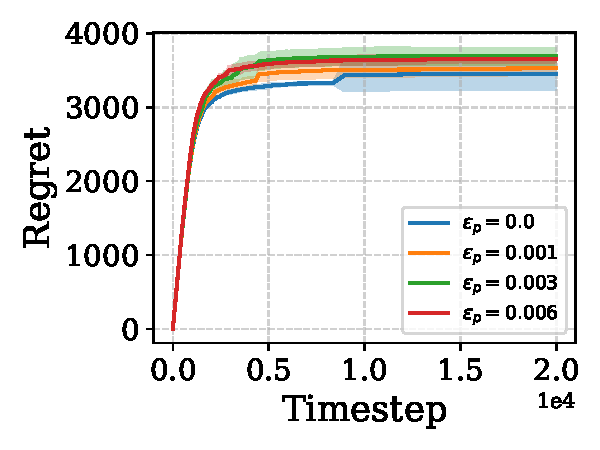
\includegraphics[width=0.4\textwidth]{images/experiment_two_gridworld.pdf}%
    \includegraphics[width=0.4\textwidth]{images/experiment_two_garnet.pdf}  
  \end{center}

\end{frame}

\begin{frame}{Experiment: Linear Speed-Up}
  \qquad \qquad \qquad \qquad GridWorld \qquad \qquad \qquad \qquad \qquad Garnet

  \vspace{-1.5em}
  
  \begin{center}
    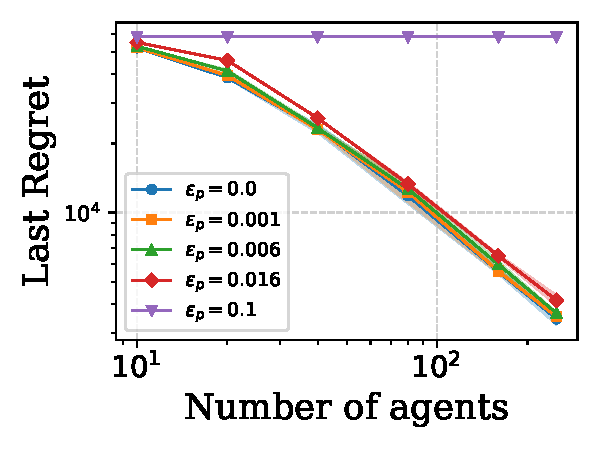
\includegraphics[width=0.4\textwidth]{images/experiment_one_gridworld.pdf}%
    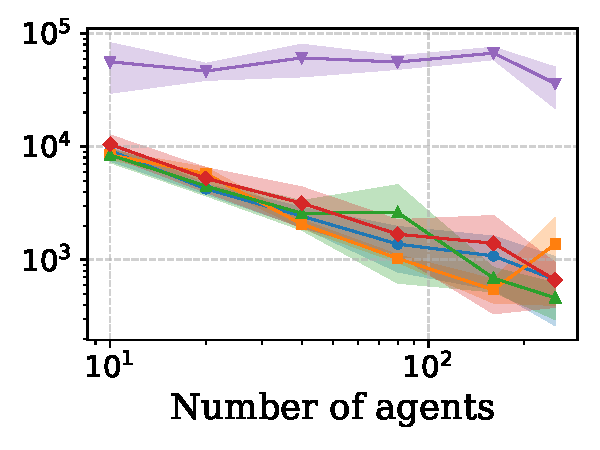
\includegraphics[width=0.4\textwidth]{images/experiment_one_garnet.pdf}  
  \end{center}
\end{frame}


\begin{frame}{Summary for Federated VI}
    \begin{itemize}
    \item We proposed federated value iteration
    \item Introduced the principle of optimism the face of heterogeneity
    \item Show that federated VI has linear speed-up!
    \end{itemize}
\end{frame}


\begin{frame}{Ongoing and Future Projects}

  \begin{itemize}
  \item federated RL:

    - analysis of federated SARSA

    - a broader benchmark of RL methods for V2X

    \vspace{0.5em}

  \item mean-field games for RL:

    - applications to telecommunications

    - analysis of actor-critic methods

    \vspace{0.5em}
    
  \item classical fedearted learning

    - revisited analysis of federated averaging

    - asynchronous federated learning
    
  \end{itemize}
\end{frame}

\begin{frame}
  \begin{center}
    \LARGE Thank you!

    \normalsize Questions?
  \end{center}
  

  \small
  See the papers:

  ~~\fullcite{mancini2024joint}

  ~~\fullcite{mangold2024scafflsa}

  ~~\fullcite{labbi2024federated}
\end{frame}

  
\end{document}
%%% Local Variables:
%%% mode: latex
%%% TeX-master: t
%%% End:
